\documentclass[12pt]{ctexart}
\usepackage[a4paper,total={6in,8in}]{geometry}
\usepackage{fancyhdr}
\usepackage[table,xcdraw]{xcolor}
\usepackage{diagbox}
\usepackage[utf8]{inputenc}
\usepackage{ctex}
\usepackage{cite}
\usepackage{color}
\usepackage{subfigure}
\usepackage{cite}
\usepackage{graphicx}
\usepackage{fontspec}
\setmainfont{Times New Roman}
\newfontfamily\timesfont{Times New Roman}
\usepackage{CJK}
\usepackage{indentfirst}
\usepackage{amsmath}
\usepackage{mathrsfs}
\usepackage{multirow}
\usepackage{svg}
\usepackage{makecell}
\usepackage{amsfonts}
\usepackage{geometry}
\usepackage{hyperref}
\usepackage{mathabx}
\usepackage{diagbox}
\usepackage{cases}
\usepackage{minipage-marginpar}
\usepackage{xcolor}
\definecolor{cherry}{HTML}{c93756}
\definecolor{tree}{HTML}{fef9d7}
% 导入包
\usepackage{hyperref}
% 格式设置
\hypersetup{hidelinks,
	colorlinks=true,
	allcolors=blue,
	pdfstartview=Fit,
	breaklinks=true}
\newcommand\dlmu[2][4cm]{\hskip1pt\underline{\hbox to #1{\hss#2\hss}}\hskip3pt}
\usepackage{fontspec} % For using system fonts with XeLaTeX or LuaLaTeX
\setmonofont{Consolas} 
    
\usepackage{listings}
    \lstset{ %
    language= MATLAB,                % choose the language of the code
    basicstyle=\footnotesize\ttfamily,       % the size of the fonts that are used for the code
    numbers=left,                   % where to put the line-numbers
    numberstyle=\footnotesize,      % the size of the fonts that are used for the line-numbers
    stepnumber=1,                   % the step between two line-numbers. If it is 1 each line will be numbered
    numbersep=5pt,                  % how far the line-numbers are from the code
    backgroundcolor=\color{tree},  % choose the background color. You must add \usepackage{color}
    showspaces=false,               % show spaces adding particular underscores
    showstringspaces=false,         % underline spaces within strings
    showtabs=false,                 % show tabs within strings adding particular underscores
    frame=single,           % adds a frame around the code
    tabsize=2,          % sets default tabsize to 2 spaces
    captionpos=b,           % sets the caption-position to bottom
    breaklines=true,        % sets automatic line breaking
    breakatwhitespace=false,    % sets if automatic breaks should only happen at whitespace
    escapeinside={\%*}{*)}          % if you want to add a comment within your code
}
    






\begin{document}

\begin{titlepage}
    \title{{\fontsize{28}{32}\selectfont\kaishu 机器人学 \\ \fontsize{20}{24}\selectfont\kaishu{作业5:运动学轨迹规划}}}
    \date{} % delete date as you want
    \maketitle
    \vspace{-7em}
    \begin{center}
      \fontsize{18}{22}\selectfont
      \textbf{\timesfont Robotics (2023-2024-2) \\
      Homework 5: Kinematic Trajectory Planning}
    \end{center}
    
    \begin{figure}[h]
        \centering
        
\includegraphics[width=0.45\textwidth]{Image/校标-校徽.png}
    \end{figure}
    \begin{center}
      \hspace{6em}
      \renewcommand{\arraystretch}{2}
      \begin{tabular}{rl}
      \fontsize{16}{50}\selectfont\heiti 姓名:& \fontsize{16}{24}\selectfont\heiti 赵四维 \\
      \fontsize{16}{24}\selectfont\heiti 学号:& \fontsize{16}{24}\selectfont 521021910696 \\
      \fontsize{16}{24}\selectfont\heiti 班级:& \fontsize{16}{24}\selectfont ME3403-01 \\
      \fontsize{16}{24}\selectfont\timesfont E-mail:& \fontsize{16}{24}\selectfont racheus.11@sjtu.edu.cn \\
      \end{tabular}
    \end{center}
    \begin{center}
      \fontsize{16}{24}\selectfont\timesfont \today
    \end{center}
\end{titlepage}

\pagenumbering{arabic}

\section{前言}
当我选上这门每个春季学期“报录比”不低于3的课程的时候,我就在心里埋下了一颗把这门课学到极致的种子。我也无数次从老师、学长们的口吻里得知这是一门“很硬”的课程,投入极大,回报未知。但我相信《机器人学》这门课程一定是我们专业通向未来的一把钥匙,一定值得去投入时间、反复钻研,一定值得和一群志同道合的朋友们一起去探讨、去实践。

4月初我们就早早地建好了我们的微信群,群名叫\textcolor{red}{RoboticsMen},显而易见,全是男生。我们在群里讨论、分享、交流,我们一起学习、一起进步。不管是令人费解的实验、还是充满未知和挑战的课程作业,大家都在群内保持高度的活跃,相互鼓励,互帮互助。从分工到选题、从建模到仿真,我们一起完成了我们本科生涯的第一门专业选修课的课程设计,留下的回忆也弥足珍贵。

本项目的第二、三章背景调研和实物建模部分由黄桢同学主要负责,孙修洁同学辅助完成。杨梓鸿同学负责了第四、第六章的选型和运动学计算部分。孙修洁同学负责了第五章的工作空间分析,以及第六章的部分调研工作。廖清淞同学负责了第七章的动力学计算和实现。我负责了第八章的运动、动力系统的模型搭建和控制仿真。最后由我和廖清淞同学、杨梓鸿同学共同完成了报告的撰写和排版工作。

5月的全力投入,6月的紧张答辩,最后用这份精美的报告作为我们这门课的完美谢幕。在这里,感谢吴建华老师和熊振华老师的悉心指导,感谢我的队友们的辛勤付出,让我留下了一段美好的回忆。

机器人学是一门伟大的学科,我常常在思考,它就像我们一直使用的PID控制器,从人力拉车到蒸汽朋克,再到如今的人工智能的盛况空前,似乎都和它有关。这门学科串联起了工业的过去、现在和未来,这门课程的结束不应该成为我们探索未至之境的终点。我相信有朝一日,我们会在建设工业强国之路上最动人的重逢。

\begin{flushright}
    \fontsize{16}{20}\selectfont\kaishu 赵四维{ \quad \quad \quad \quad}\\
    \fontsize{16}{20}\selectfont\kaishu 2024年6月23日
\end{flushright}


\newpage
\tableofcontents


\newpage
\pagestyle{fancy}
\fancyhf{}
\fancyhead[L]{ME3403-01}
\fancyhead[C]{基于ABB-IRB-1200的协作机器人课程设计}
\fancyhead[R]{2023-2024-2}
\fancyfoot[C]{\thepage}

% PART I Chapter1-4 
\section{协作机器人的现状和发展状况调研}
协作机器人(Collaborative Robot,简称Cobot)作为一种新兴的机器人品类,因其设计初期就考虑了降低伤害风险、能安全地与人类进行直接交互和接触,具有轻量化、灵活性高、安全可靠、简单易上手、便于部署等特点,近年来在全球范围内迅速发展,从它的英文名中就可以看出它是一种协助劳动的机器人,相比于死板、重复性工作的传统工业机器人,协作机器人可以说是工业机器人的升级,借助全新的交互技术让人可以在协作机器人的帮助之下一同完成任务。

全球协作机器人的发展从1996年正式开始,协作机器人“COBOT”的概念由美国首次提出,并申请了该领域的首个专利,在2008年UR公司推出了全球首款协作机器人 UR5,在2012年Rethink Robotics 公司推出了一款双臂协作机器人Baxter,从2013年到2015年,传统工业机器人四大家族开始涉足协作机器人领域,在2015年,国内的协作机器人如雨后春笋般出现,新松机器人,推出了国内首台自主研发的七轴协作机器人,遨博智能发布了一款轻型协作机器人AUBO-i5。

我国不断支持机器人产业的发展,提出多项相关政策,从2015年的《中国制造2025》、2016年机器人产业被写入“十三五”规划、2021年出台《“十四五”机器人产业发展规划》、2023年出台《“机器人+”应用行动实施方案》,我国不断推进机器人产业发展,走向机器人技术世界前列。

根据Emergen研究,全球协作机器人市场规模预计到2027年将达到93.428亿美元,并在整个预测期内实现38.5\%的复合年增长率。中国市场也表现出强劲的增长势头,2022年市场规模约为26.79亿元,占全球总销量的四成以上,呈现明显的进口替代趋势。预计到2028年,协作机器人市场的复合年增长率将达到30\%,市场将持续扩张。全球协作机器人市场预计将以42\%的速度增长,从2019年的6.803亿美元增长到2027年的93.428亿美元。

协作机器人的核心技术要素包括易用性、灵活性、安全性和共融性。这些技术使得协作机器人能够与作业环境、与人及其它机器人自然交互,可以自主适应复杂动态环境并进行有效协作。主要技术发展方向包括智能感知、自主认知、人机交互和碰撞检测等。协作机器人在汽车制造、电子、食品和饮料、塑料和聚合物、家具和设备、医疗和物流等行业有广泛应用。其中,负载能力在10kg以上的协作机器人增速最快。

未来协作机器人将更加注重智能化和自主性。研究人员预计将能够识别人类的基本行为,并调整这些机器人的行为以更好地与人类合作。此外,共融机器人将成为未来发展趋势,它们能与作业环境、与人及其它机器人自然交互,可以自主适应复杂动态环境并进行有效协作。

\section{机器人建模}
\subsection{三维建模}
使用SolidWorks软件进行建模,参照ABB IRB1200型号的协作机器人进行设计,在3D建模设计过程中不考虑电机位置和走线,在建模完成之后根据具体建模尺寸进行分析。

ABB-IRB-1200型号机器人是一款小型协作机器人,可以实现在工作工程当中和人相互合作,实现人机交互,在设计过程中减少棱角,对人体进行保护。我们在完成自己设计的过程当中,参考了这一款机器人的基本形状,并对其中的棱角部分进行优化,对尺寸大小进行调整,获得最适合我们后续数学建模和仿真分析的6自由度机器人。

\begin{figure}[h]
    \centering
    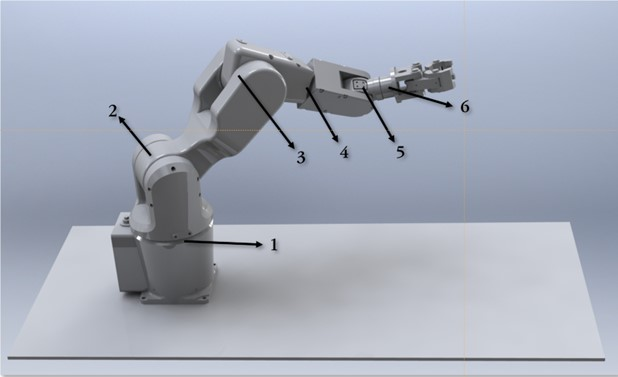
\includegraphics[width=0.8\textwidth]{Image/fig1.jpg}
    \caption{机器人模型和各自由度关节示意图}
    \label{fig:1}    
\end{figure}

我们设计的机器人模型如图\ref{fig:1}所示,可以看到一共7个部分,相互组合一共产生6个自由度,自由度2、3、5为绕水平轴旋转的自由度,自由度1、4、6为绕垂直轴旋转的自由度。最后6个自由度的角度变化驱动最后加持部件的运动,我们的加持部件最后采用了机械夹取手的形式,用来做出灵活的运动,机械夹取手的具体细节如图\ref{fig:2}所示。

\begin{figure}[h]
    \centering
    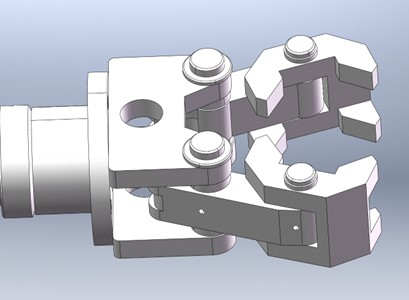
\includegraphics[width=0.8\textwidth]{Image/fig2.jpg}
    \caption{机械夹取手的设计}
    \label{fig:2}
\end{figure}

\subsection{简单运动模拟}
在完成机械臂的建模之后,我们需要模拟机械臂是否已经完成约束配合,能否通过6个自由度上的角度变动带来最后机械臂的自由运动。我们使用了SolidWorks当中的SolidWorks Motion插件,通过这个插件可以让机械臂的末端按照我们规划好的路线运动。我们规划了一个水平圆,让机械臂末端的一个固定点和这个圆进行路径配合,让机械臂的末端绕着这个圆运动。之后利用SolidWorks Motion插件,为这个运动增加了一个路径匹配电机,让机械臂按照制定位置运动。但是也会出现一个问题,机械臂在运动时并没有解决干涉问题。在运动过程中可能存在干涉,导致机械臂出现重合的奇怪现象。目前没有办法能够解决,只能通过调整机械臂的起始姿态和后续的运动距离来避免机械臂重合的现象。

\subsection{运动模拟仿真渲染}
SolidWorks中自带的渲染软件无法完成我们需要的运动渲染,最后我们使用了Keyshot软件。将SolidWorks中已经做好的路径规划导出到Keyshot中,再完成相机布置和运动、背景布置最终完成运动渲染仿真,渲染仿真动画截图如图\ref{fig:3}所示。

\begin{figure}[h]
    \centering
    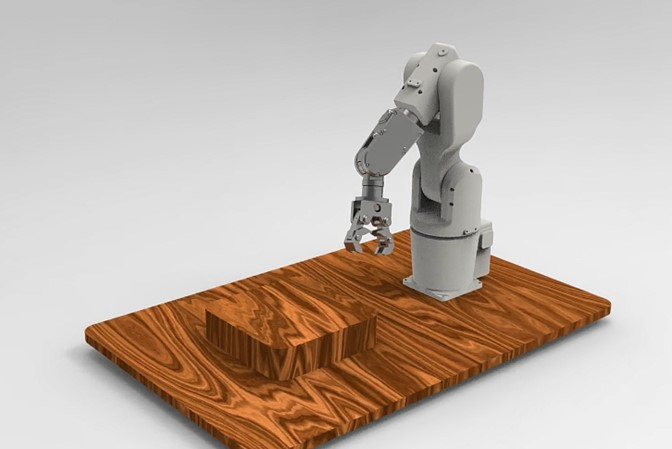
\includegraphics[width=0.8\textwidth]{Image/fig3.jpg}
    \caption{运动仿真渲染}
    \label{fig:3}
\end{figure}

\subsection{应力仿真分析}
最先采用SolidWorks中的Simulation模块进行应力分析,但是在SolidWorks中容易出现网格无法划分的现象,最后使用ANSYS中的静态结构进行应力分析,机械臂的最终采用使用铝合金,因为铝合金具有更轻的重量和比较好的力学表现。在测量机械臂的应力时,我们考虑将机械臂完全伸直,将机械臂在XY平面中伸展到最远,让夹持端受到压力时带来的力矩最大,模拟在最坏的情况下的机械臂应力和形变情况。模拟情况如图\ref{fig:4}所示,红色为受压力较大的地方,颜色越深受到的压力越大,从应力分析的图中可以看到在较细的地方会有更大的应力。

\begin{figure}[h]
    \centering
    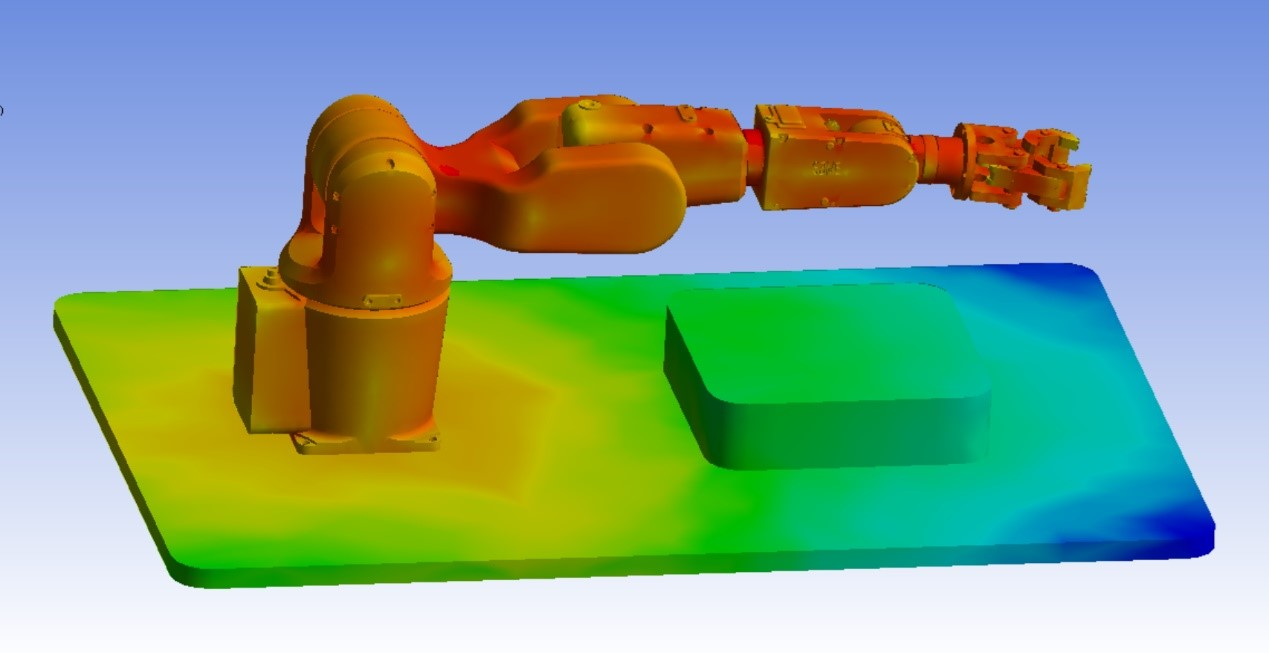
\includegraphics[width=0.7\textwidth]{Image/fig4.jpg}
    \caption{应力分析仿真模拟图}
    \label{fig:4}
\end{figure}

我们还对变形大小进行了分析,模拟情况如图\ref{fig:5}所示,可以看到末端相对于原先位置的位移最大。可以看到最大的变形为0.033472mm,我们可以根据这个数据去计算出位置误差。

\begin{figure}[h]
    \centering
    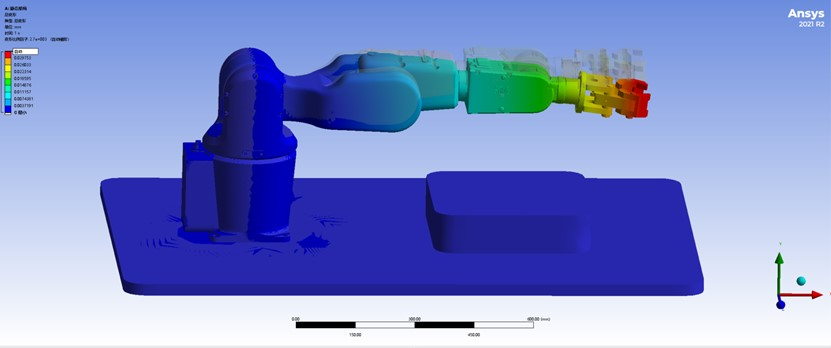
\includegraphics[width=0.7\textwidth]{Image/fig5.jpg}
    \caption{变形分析仿真模拟图}
    \label{fig:5}
\end{figure}

\subsection{误差分析}
在实际应用中,很多因素会影响到机械臂的绝对定位精度,按照定位误差的来源来分类,包括外界环境的变化引起的外部误差和内部结构参数引起的内部误差。

我们调研的结果主要有:
\begin{enumerate}
    \item 结构刚度和变形:
    
    自重:机械臂各个部件的自重会导致结构的弯曲和变形,特别是在机械臂的末端部分,这种效应会更加明显。自重引起的重力作用会使关节和连杆产生变形,导致位置和姿态的误差。

    外力和惯性力:工作过程中受到的外力(如负载和加工力)以及运动时的惯性力也会引起结构变形,导致误差。

    \item 关节误差:
    齿轮传动误差:如果机械臂使用齿轮传动,各个齿轮的制造误差、安装误差和磨损会导致传动精度降低。

    关节间隙:关节中的轴承和传动装置存在间隙,这些间隙在运动过程中会积累误差。

    伺服电机控制精度:电机的控制精度(如分辨率和响应速度)直接影响关节的定位精度。

    \item 传感器误差:
    
    位置传感器精度:用于测量关节角度或位置的传感器(如编码器或电位计)的分辨率和精度会影响定位精度。

    噪声和干扰:传感器信号在传输过程中可能受到电磁干扰和噪声的影响,导致测量数据不准确。
\end{enumerate}

除了以上三种主要的干扰外,误差还来自外界环境的变化包括工作环境中的温度、湿度的变化,电网的冲击,通讯信号的干扰,其他设备的振动,人为因素的干预等;内部由机械臂自身某些部分引起的误差,包括机械臂的运动学参数误差、运动时的摩擦磨损以及润滑条件等。

综合分析以上误差来源,外界环境的变化、受力变形、摩擦磨损等对机械臂的绝对定位精度影响较小,机械臂的运动学参数误差影响较大,由其所导致的误差约占总误差的80\%。

虽然机械臂的定位误差产生原因很多,在理论分析过程中,目前我们能够做到的只有分析机械臂自重所带来的位置误差0.033472mm,这个误差相对于机器人自身的以米为单位的大小这个误差很小,并且我们的重力按照实心重力计算,在使用空心合理优化的情况下机器人自身重量带来的误差会更小。

通过误差传递方程,考虑每一个误差源对于最终结果的敏感性,创建函数:
\begin{equation}
    \varDelta f=\sqrt{\left( \frac{\partial f}{\partial x_1}\Delta x_1 \right) ^2+\left( \frac{\partial f}{\partial x_2}\Delta x_2 \right) ^2+\cdots +\left( \frac{\partial f}{\partial x_n}\Delta x_n \right) ^2}
\end{equation}

这里,$\frac{\partial f}{\partial x_i}$是$f$对$x_i$的偏导数, $\Delta x_i$是$x_i$的误差。从公式中可以看到随着产生误差变量的增多,系统的误差会逐渐增大,并且相对于不同的误差,会有不同的计算权重来进行叠加。以简单的双关节机械臂来看,假设其两个关节角分别为$\theta_1,\theta_2$连杆长度分别为$l_1,l_2$,由末端位置可以得到正向运动学方程,

\begin{equation}
    \left\{ \begin{array}{c}	x=l_1cos\left( \theta _1 \right) +l_2cos\left( \theta _1+\theta _2 \right)\\	y=l_1sin\left( \theta _1 \right) +l_2sin\left( \theta _1+\theta _2 \right)\\\end{array} \right. 
\end{equation}

假设角度和长度都存在误差$\Delta\theta_1,\Delta\theta_2,\Delta l_1,\Delta l_2$,则根据误差传递函数可以得到统计结果:

\begin{equation}
    \begin{aligned}
    \varDelta x &=\sqrt{\left( \frac{\partial x}{\partial \theta _1}\Delta \theta _1 \right) ^2+\left( \frac{\partial x}{\partial \theta _2}\Delta \theta _2 \right) ^2+\left( \frac{\partial x}{\partial l_1}\Delta l_1 \right) ^2+\left( \frac{\partial x}{\partial l_2}\Delta l_2 \right) ^2}\\
    \varDelta y &=\sqrt{\left( \frac{\partial y}{\partial \theta _1}\Delta \theta _1 \right) ^2+\left( \frac{\partial y}{\partial \theta _2}\Delta \theta _2 \right) ^2+\left( \frac{\partial y}{\partial l_1}\Delta l_1 \right) ^2+\left( \frac{\partial y}{\partial l_2}\Delta l_2 \right) ^2}
    \end{aligned}
\end{equation}

通过这些计算就可以得到最终的误差,通过识别不同的误差源并且建立适当的误差传递方程就可以得到能正确反映机器人误差的方程。对于我们的六自由度协作机器人,我们的单一误差就能达到12个,再加上不同关节角度和连杆长度所产生的误差也是由其他的误差叠加产生,就会产生一个非常复杂的误差传递方程。

想要减少误差我们可以采用一下几种办法:

\begin{itemize}
    \item 采用高刚度材料和结构设计,减少变形,针对由于自重变形部分的误差进行误差减小。
    \item 提高传动装置和传感器的制造和装配精度,通过对装配误差的控制,减小不可控的精度差。
    \item 使用补偿算法,校正因温度变化和其他因素引起的误差,通过误差补偿,直接针对系统的误差进行校正。
    \item 优化控制算法,提高控制系统的响应速度和稳定性,同时可以减小运动过程中对于机械臂的磨损,让精度长时间保存。
    \item 定期维护和校准机械臂,确保其各部分处于最佳状态,对其中影响误差的部分进行修复确保精度正确。
\end{itemize}

以上方法可以通过控制误差方程中的一个或者多个误差来减小整体的误差,对于误差的调整程度需要对于实际的机器人进行具体的分析。

\section{材料与选型}
\subsection{材料选择}
材料选择方面,我们收集了市面上常见机器人材料的资料,其优缺点对比情况如\ref{fig:6}所示。在各连杆材料选择时,我们需要综合考虑材料密度、刚度、强度、成本等多方面因素。

\begin{figure}[h]
    \centering
    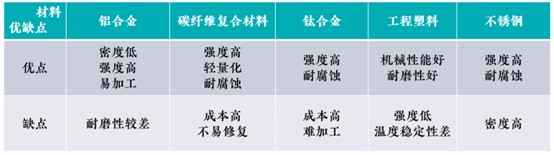
\includegraphics[width=0.7\textwidth]{Image/fig6.jpg}
    \caption{常见机器人材料优缺点对比}
    \label{fig:6}
\end{figure}

最终我们选取了不锈钢作为底座,其具有足够的强度和密度,足以稳定机身;选取了中空的铝合金作为机器人杆件、关节的材料,该材料能兼顾强度、刚度、重量,且中空的结构使机器人从法兰到底座能够全程内部走线。

\subsection{电机、减速器选型}
考虑到机器人关节速度不能过大,统一电机的额定转速为3000 r/min,故初步选取减速比i=100的谐波减速机。	

在机器人末端施加6kg负载,通过动力学的计算,可得出机器人需要的额定转矩估值,以此为依据为机器人各关节选取合适的电机和减速机。

选取结果如表\ref{tab:1}所示:

\begin{table}[h]
    \centering
    \caption{电机、减速器选型}
    \label{tab:1}
    \vspace{5pt}
    \begin{tabular}{cccccc}
    \rowcolor[HTML]{4472C4} 
    关节 & \begin{tabular}[c]{@{}c@{}}额定转矩\\ (Nm)\end{tabular} & \begin{tabular}[c]{@{}c@{}}减速机型号\\ (i=100)\end{tabular} & \begin{tabular}[c]{@{}c@{}}额定转矩\\ (Nm)\end{tabular} & 电机型号             & \begin{tabular}[c]{@{}c@{}}电机额定功率\\ (Nm)\end{tabular} \\
    \rowcolor[HTML]{D9E2F3} 
    1  & 60                                                  & SHXB-CSF-25-A                                           & 0.6                                                 & SM 60-006-30 LFB & 0.2                                                   \\
    2  & 67                                                  & SHXB-CSF-25-A                                           & 0.67                                                & SM 60-006-30 LFB & 0.2                                                   \\
    \rowcolor[HTML]{D9E2F3} 
    3  & 30                                                  & SHXB-CSF-20-A                                           & 0.3                                                 & SM 40-003-30 LFB & 0.1                                                   \\
    4  & 65                                                  & SHXB-CSF-25-A                                           & 0.65                                                & SM 60-013-30 LFB & 0.4                                                   \\
    \rowcolor[HTML]{D9E2F3} 
    5  & 100                                                 & SHXB-CSF-32-A                                           & 1                                                   & SM 80-013-30 LFB & 0.4                                                   \\
    6  & 60                                                  & SHXB-CSF-25-A                                           & 0.6                                                 & SM 60-006-30 LFB & 0.2                                                  
    \end{tabular}
    \end{table}
    
    图\ref{fig:7}展示了我们选用的主要型号的减速器的工程图,图\ref{fig:8}展示了我们选用的主要型号的电机实物图。
\begin{figure}[h]
    \centering
    \subfigure[减速器工程图]{
    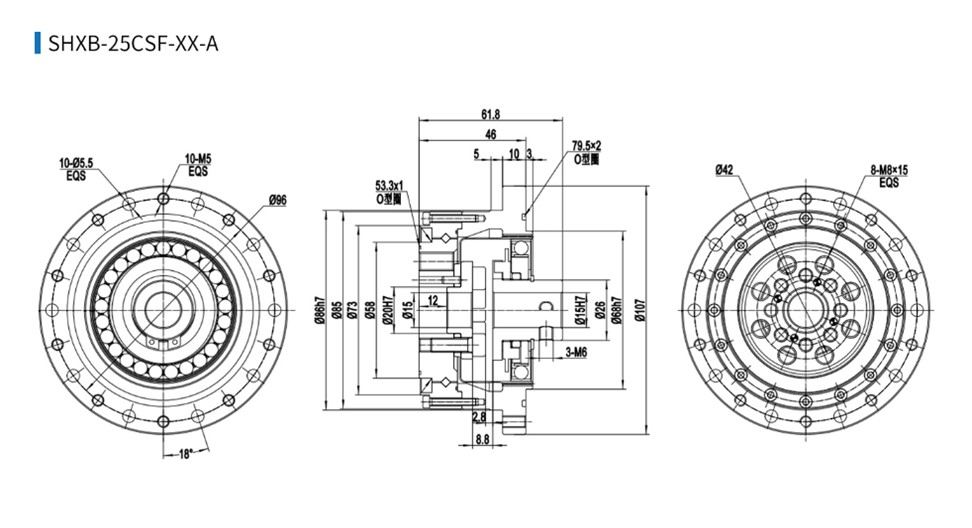
\includegraphics[width=0.5\textwidth]{Image/fig7.jpg}
    \label{fig:7}
    }
    \subfigure[电机实物图]{
    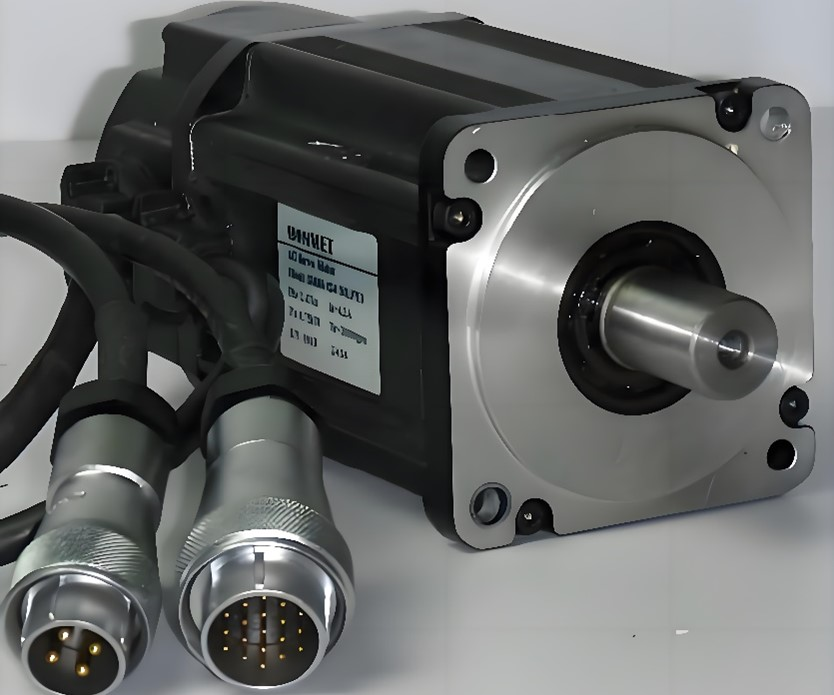
\includegraphics[width=0.4\textwidth]{Image/fig8.jpg}
    \label{fig:8}
    }
    \caption{减速器和电机选型}
\end{figure}
\newpage

\section{工作空间}
\subsection{背景介绍}
机器人的工作空间是评价机器人工作性能的一项重要指标。工作空间分为可达工作空间和灵巧工作空间。可达工作空间是指机器人末端执行器参考点所能到达的位置的集合。

机器人工作空间是机器人设计与优化的重要依据。王晓华等以六轴缝纫机器人为对象,通过对机器人末端的可达工作空间分析确定了缝纫机器人在工作时各关节的最佳运动范围。荆学东等以六轴双臂服务机器人为对象,求解了双臂各自的可达工作空间,以协作空间最大为优化目标,对机器人的结构参数进行了优化。赵智远等研制了 9 自由度超冗余串联机械臂,以可达工作空间与灵活工作空间为优化目标,对机械臂的构型进行了优化设计。贾世元等以六轴机械臂为对象,以全局灵活性为优化目标,对机械臂尺寸参数进行了优化设计。

目前,求解机器人工作空间的方法主要有3类:几何法、解析法和数值法:
\begin{itemize}
    \item \textbf{几何法}可以得到机器人的解剖面或解剖线,但受到自由度数的限制,无法精确描述多自由度机器人的工作空间,主要用于平面机器人的求解。
    \item \textbf{解析法}是通过多次包络求解机器人工作空间的方法,可以求出工作空间边界的数学方程,但求解过程复杂,主要用于关节数量少于3个的机器人。
    \item \textbf{数值法}是将多个关节角组合代入到正向动力学方程,求解出机器人末端在任务空间的坐标,最终得到工作空间的方法,求解简单,适用于任意结构的机器人工作空间的求解。
\end{itemize}

在数值方法中,求解机器人工作空间最为常见的方法就是蒙特卡洛方法。传统蒙特卡洛法的主要问题是工作空间点分布不均匀,大部分工作空间点产生在工作空间内部,导致工作空间边界求取精度不高,当提高工作空间点数量以提升工作空间边界求取精度时,大量工作空间点任然出现在工作空间内部,造成了计算资源的浪费,导致求解速度较慢。针对上述问题,徐振邦等利用蒙特卡洛法生成了一个种子工作空间,对于每个工作空间点数量较少的位置,在其内部选取一个参考点,在生成该点的关节角附近多次随机抽样并代入正向运动学方程,一次性得到多个工作空间点。这种方法使工作空间点云密度分布更加均匀,提高了工作空间边处的精确度,但该方法的求解效率与分块数有关,需要根据具体的结构进行调整,并且拓展得到的工作空间点过于集中。刘志忠等先利用蒙特卡洛法生成了一个种子空间,对种子空间分层,寻找每层的边界点,在边界点附近生成多个随机点,多次迭代,直到形成精确的边界。这种方法提高了工作空间边界处的精度,但求解精度依赖于分层数量,分层过少时精度不高,分层过多时消耗时间长。

在本项目中,我们参考李星辰提出的改进的蒙特卡洛方法,利用传统蒙特卡洛法生成种子空间,拓展随机点数量较少的子空间,动态调整正态分布概率密度函数的参数,得到了可达工作空间。

\subsection{传统Mento Carlo方法}
蒙特卡洛法是一种基于概率统计理论,用于模拟随机现象的数值方法。在求解机器人工作空间时,在各个关节角取值范围内随机抽取大量的关节角变量值进行组合,将这些关节角值组合带入正向运动学方程,计算出机器人末端执行器参考点的坐标值,这些参考点所包络的空间就是机器人工作空间。

传统蒙特卡洛法存在的问题如下:求解机器人工作空间时,工作空间边界的具体位置由工作空间边界的参考点给出,工作空间内部的点意义不大。然而,虽然传统蒙特卡洛法随机抽取的关节角值服从均匀分布,但关节空间到工作空间的映射是非线性的,大量工作空间点出现在工作空间内部,导致工作空间的精度不高。当增加随机抽取的关节角值组合的数量时,大部分参考点任然出现在非工作空间边界部分,虽然工作空间的精度变高,但大量的工作空间点没有意义,造成了计算资源的浪费。

\subsection{改进Mento Carlo方法}
针对上述问题,我们再项目中提出一种改进的蒙特卡洛法,该方法由3个部分组成:
\begin{enumerate}
    \item 生成种子空间。利用传统蒙特卡洛法生成大量的工作空间点,用长方体包络所用种子空间点,划分成数个相等的子空间。
    \item 拓展种子空间。筛选出需要拓展的子空间,利用正态分布抽样对这些子空间拓展,同时设置一个精度阈值确保拓展后的工作空间足够准确。为了保证拓展产生的点出现在边界附近,正态分布概率密度函数的方差会根据拓展后的点的位置进行调整。 
    \item 输出可达工作空间。多次重复拓展过程,直到每个子空间得到精确描述,输出可达工作空间。
\end{enumerate}

工作流程图可参考图\ref{fig:9}。

\begin{figure}[h]
    \centering
    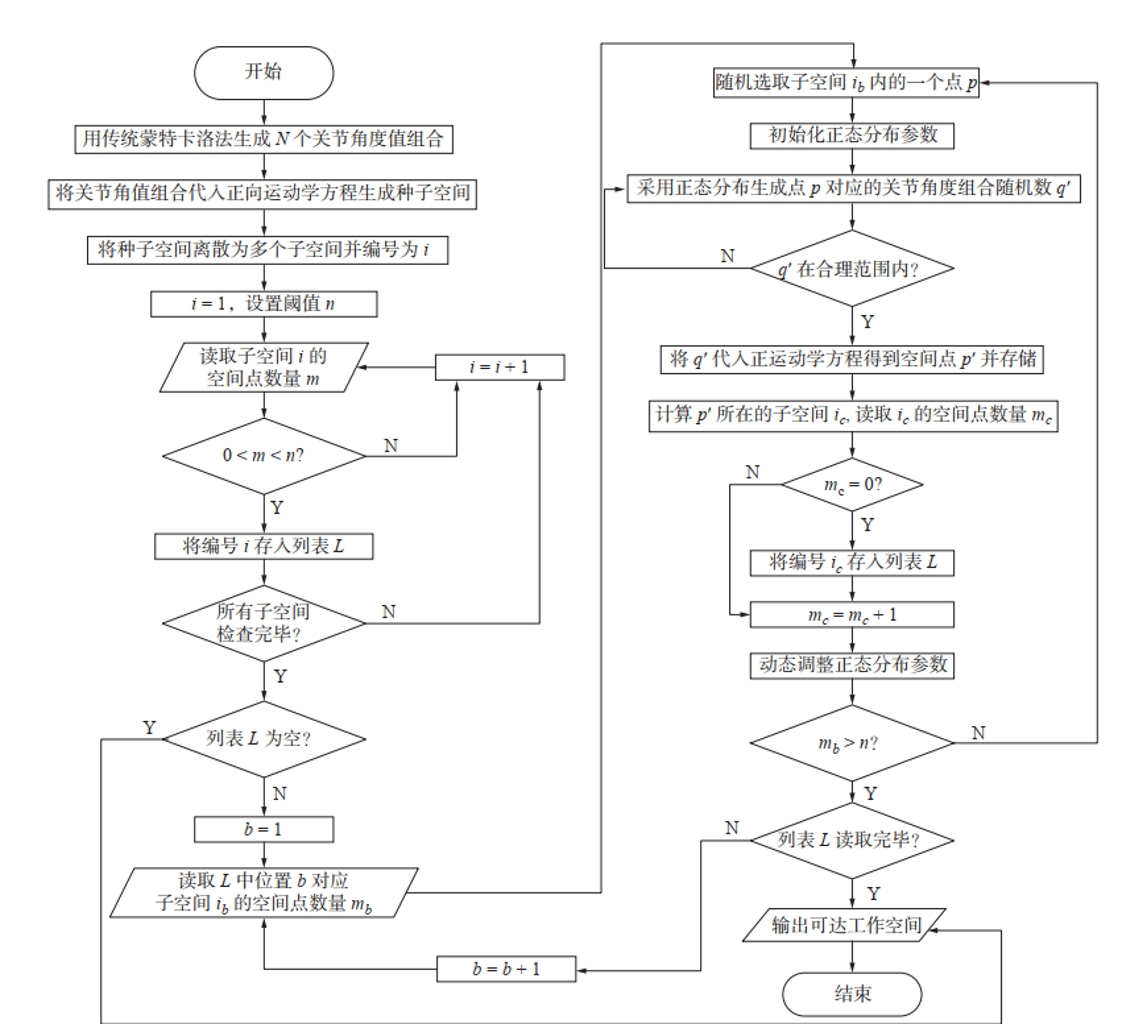
\includegraphics[width=0.8\textwidth]{Image/fig9.jpg}
    \caption{改进Menlo Carlo方法工作流程图}
    \label{fig:9}
\end{figure}

具体的详细步骤如下:
\newpage
\begin{enumerate}
    \item \textbf{生成种子空间} 
    
    用传统蒙特卡洛法对每一关节生成N个随机角度值,按序号组成对应关节角值组合。将关节角值组合代入正向运动学方程,求解出工作空间点在三维笛卡尔坐标系中的坐标值 ,记录参考点在3个坐标轴方向的最大值和最小值,并分别表示为$X_{max},X_{min},Y_{max},Y_{min},Z_{max},Z_{min}$。
    
    将求得的长方体分别沿 3 个坐标轴方向分成$n_x,n_y,n_z$等距部分,整个长方体被分成了$k=n_x\times n_y\times n_z$ 个相等的子空间,根据每个子空间的位置进行编号,存储每个子空间内的工作空间点数量$m$,并存储每个工作空间点的位置信息以及关节角信息。
    \item \textbf{拓展种子空间}
    
    为了在提高可达工作空间边界求取精度时,减少计算资源的浪费,并且方便灵活工作空间的求解,应对每个工作空间点数量较少的子空间进行拓展。设置工作空间点数量阈值$n$,对每个子空间判断,若子空间内包含工作空间点并且工作空间点数量$<n$,则该子空间需要拓展,将该子空间的编号存入列表$L$;否则,不存入列表。所有子空间检查完毕后,对列表$L$进行判断,若列表$L$不为空,则对所有与列表$L$中编号对应的子空间进行拓展;否则,输出可达工作空间。
    
    对每一个需要拓展的子空间$i$,随机抽取一个该子空间内部的工作空间点p,找到与该点对应的关节角值组合q。在关节角值组合$q$附近利用正态分布概率密度函数选取随机值,均值$\mu=q$,标准差初始值依据具体情况进行设定。取值后对新空间点的合理性进行判断,若关节角值组合q的每个关节角值都在该关节角的取值范围内,则保留该取值;若不满足,则舍弃该次取值并重新取值。将取得的关节角值组合$q\prime$代入正向运动学方程,产生一个新的工作空间点$p\prime$,并存储新生成工作空间点的位置信息和关节角信息。为了使得每个本应存在工作空间点的子空间均得到拓展,计算出工作空间点$p\prime$所在的子空间$i_c$,读取子空间$i_c$的工作空间点数量$m_c$,对其进行判断,若$m_c=0$,则将子空间存入列表$L$。为了避免拓展后的工作空间点集中出现在一个工作空间点附近,每拓展一次后进行判断,若该子空间中的工作空间点数量小于阈值$n$,则重新在该子空间中的工作空间点中任意抽取一个点$p$,重复拓展过程,直到该子空间中的工作空间数量大于阈值$n$。

    由于部分子空间与实际工作空间的交集较小,在拓展这一类子空间时,新生成的点$p\prime$虽然大部分出现在被拓展点$p$附近,却出现在被拓展点$p$所在的子空间之外,导致该子空间附近的子空间产生大量的工作空间点,造成了计算资源的浪费。同时,部分位于关节角范围边界处的关节角值组合q,在产生新的关节角值组合$q\prime$时,$q\prime$常常出现在关节角取值范围外,需要重新取值,造成了资源的浪费。为了减少上述的计算资源的浪费,需要根据新生成的关节角值$q\prime$和工作空间点$p\prime$的位置调整正态分布的方差$\sigma$。用$n_f$代表拓展时新生成的关节角值在对应关节角取值范围外的次数,用$n_l$代表拓展时新生成的工作空间点出现在被拓展点p所在子空间外的次数,当$n_f$大于临界值$n_f^{max}$时,表明正态分布方差$\sigma$过大,将正态分布方差$\sigma$除以一个大于1的数$\delta$以缩小方差$\sigma$,方差$\sigma$调整后,将$n_f$置零;当$n_l$大于临界值$n_l^{max}$时,表明该子空间与实际工作空间的交集较小,将正态分布方差$\sigma$除以一个大于1的数$\delta$以缩小方差$\sigma$,方差$\sigma$调整后,将$n_l$置零。每拓展完一个子空间后,$n_f,n_l$置零。
    \item \textbf{输出可达工作空间}
    
    列表L中的子空间全部拓展后,每个子空间已得到精确描述,得到可达工作空间,输出存储的点的位置信息。
\end{enumerate}

\subsection{实例求解}
基于我们小组的机械臂模型参数,我们分别用传统蒙特卡洛法和本文所述的改进蒙特卡洛法在 MATLAB 编程,进行工作空间求解仿真,并利用 MATLAB 中的拟合函数求解工作空间体积。

首先设置改进的蒙特卡洛法参数,如表\ref{tab:2}所示:

\begin{table}[h]
    \centering
    \caption{改进蒙特卡洛法参数设置}
    \vspace{5pt}
    \label{tab:2}
    \begin{tabular}{
    >{\columncolor[HTML]{ECF4FF}}c 
    >{\columncolor[HTML]{ECF4FF}}c 
    >{\columncolor[HTML]{ECF4FF}}c 
    >{\columncolor[HTML]{ECF4FF}}c 
    >{\columncolor[HTML]{ECF4FF}}c 
    >{\columncolor[HTML]{ECF4FF}}c 
    >{\columncolor[HTML]{ECF4FF}}c }
    \hline \hline
    N     & k        & n  & $\sigma$ & $\delta$ & $n_f^{max}$ & $n_l^{max}$ \\ \hline
    10000 & 20*20*20 & 50 & $\pi/3$  & 1.5      & 5           & 300         \\ \hline\hline
    \end{tabular}
    \end{table}

其中,N是初始生成的种子数,k是划分的子空间的数量,n是设置的工作子空间点数量阈值,$\sigma$是方差,$\delta$是一个大于1的参数,$n_f^{max}$新生成的关节角值在对应关节角取值范围外的次数的最大值,$n_l^{max}$新生成的工作空间点出现在被拓展点p所在子空间外的次数的最大值。

\textbf{下面进行相同工作空间点数下的比较}:下面四张图片分别展示了传统的蒙特卡洛方法与改进的蒙特卡洛方法求解的工作空间的示意图,可以清楚的看到,在生成的工作点数均为$1000000$左右的情况下,传统的蒙特卡洛方法生成的工作空间的边界粗糙、模糊、像是像素低一般,而改进的蒙特卡洛方法生成的工作空间的边界圆润、清晰,效果较好。

\begin{figure}[h]
    \centering
    \subfigure[传统蒙特卡洛法工作空间示意图1]{
    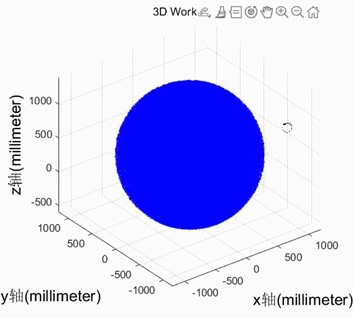
\includegraphics[width=0.4\textwidth]{Image/fig10.jpg}
    }
    \subfigure[传统蒙特卡洛法工作空间示意图2]{
    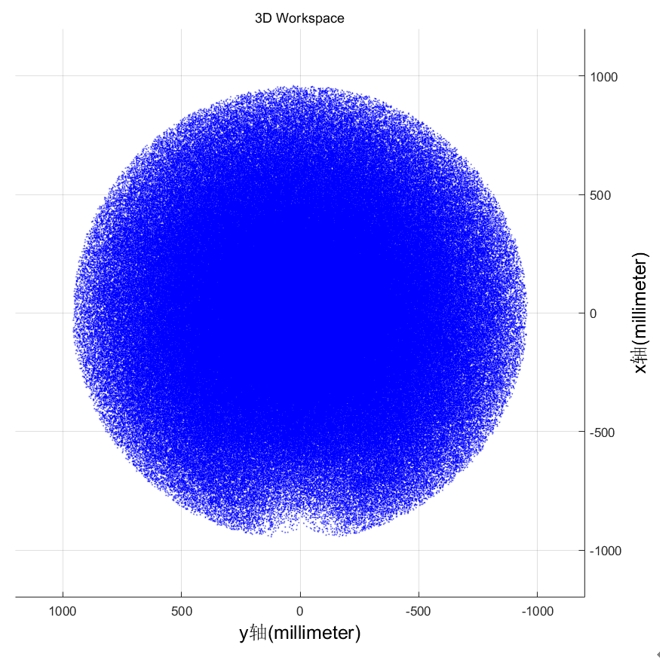
\includegraphics[width=0.4\textwidth]{Image/fig11.png}
    }
    \caption{传统蒙特卡洛法工作空间示意图}
    \label{fig:10}
\end{figure}


\begin{figure}[h]
    \centering
    \subfigure[改进蒙特卡洛法工作空间示意图1]{
    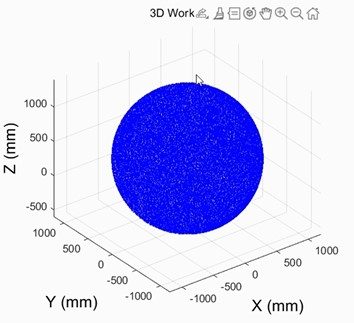
\includegraphics[width=0.4\textwidth]{Image/fig12.jpg}
    }
    \subfigure[改进蒙特卡洛法工作空间示意图2]{
    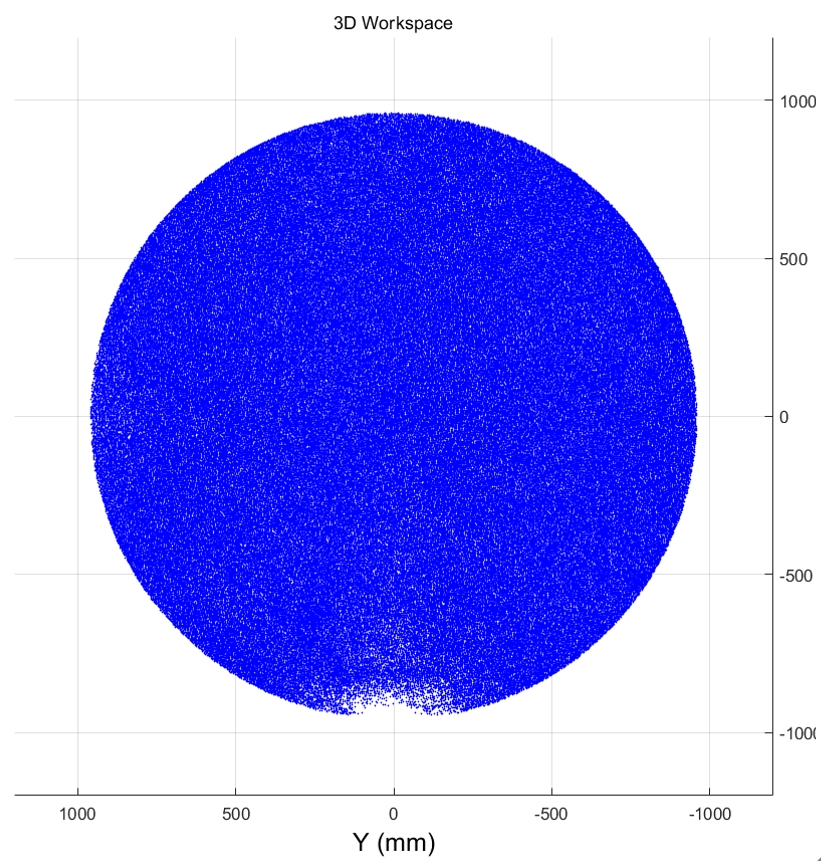
\includegraphics[width=0.4\textwidth]{Image/fig13.jpg}
    }
    \caption{改进蒙特卡洛法工作空间示意图}
    \label{fig:11}
\end{figure}

\textbf{对不同空间工作点数下传统的蒙特卡洛方法进行比较}:

通过不断增加传统蒙特卡洛法的随机工作空间点数量,使求解得到的工作空间越来越接近实际工作空间。用生成的工作空间体积变化表示工作空间的变化,逐渐增加工作空间点数量,工作空间的体积随工作空间点数量增加的变化如表\ref{tab:3}所示:

\begin{table}[h]
    \centering
    \caption{传统方法求得的可达工作空间体积随工作空间点数数量的变化}
    \vspace{5pt}
    \label{tab:3}
    \begin{tabular}{
    >{\columncolor[HTML]{FFFFC7}}c |
    >{\columncolor[HTML]{FFFFC7}}c |
    >{\columncolor[HTML]{FFFFC7}}c |
    >{\columncolor[HTML]{FFFFC7}}c |
    >{\columncolor[HTML]{FFFFC7}}c |
    >{\columncolor[HTML]{FFFFC7}}c |
    >{\columncolor[HTML]{FFFFC7}}c |
    >{\columncolor[HTML]{FFFFC7}}c }
    \hline \hline
    N       & $5000$ & $10^4$ & $5\times 10^4$ & $10^5$ & $5\times 10^5$ & $10^6$ & $10^7$ \\ \hline
    $V/m^3$ & 3.3486 & 3.4374 & 3.5791         & 3.6104 & 3.6615         & 3.6740 & 3.6950 \\ \hline \hline
\end{tabular}
\end{table}

从表\ref{tab:3}可以看出,当工作空间点数达到1000000时,体积不再明显变化,体积为3.6950 $m^3$;采用改进方法求解,当体积达到3.6947$m^3$时,仅需要422458个工作点,所以需要的点数仅为传统方法的4.22\%,求解效率大大提高。

传统的蒙特卡洛方法生成的工作空间的边界如图\ref{fig:10}所示,改进的蒙特卡洛方法生成的工作空间的边界如图\ref{fig:11}所示,可以看出改进的蒙特卡洛方法生成的工作空间的边界更加清晰、圆润,效果更好。

对于不同点数的工作空间的示意图如图\ref{fig:12}所示,可以看出,随着工作空间点数的增加,工作空间的边界越来越清晰,更加接近实际工作空间,出于实际排版美观的考虑,将图片放在下页。

\begin{figure}[htbp]
    \centering
    \subfigure[$N=5000$]{
    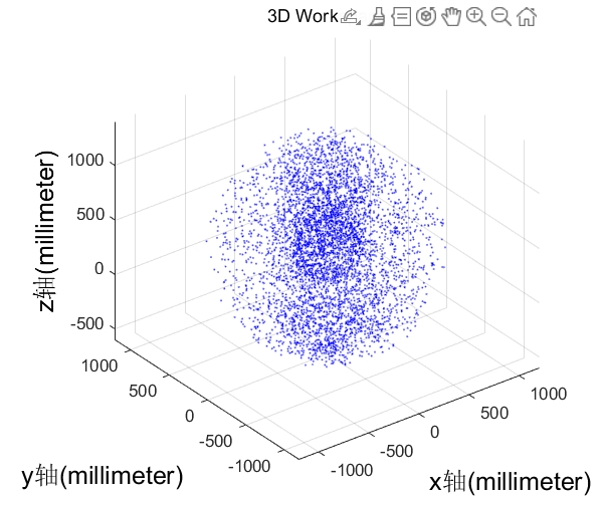
\includegraphics[width=6cm]{Image/fig14.jpg}
    }
    \quad
    \subfigure[$N=10^4$]{
    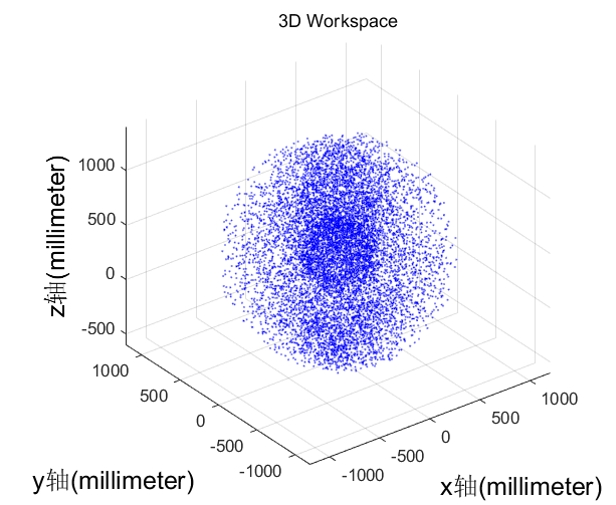
\includegraphics[width=6cm]{Image/fig15.jpg}
    }
    \quad
    \subfigure[$N=5\times 10^4$]{
    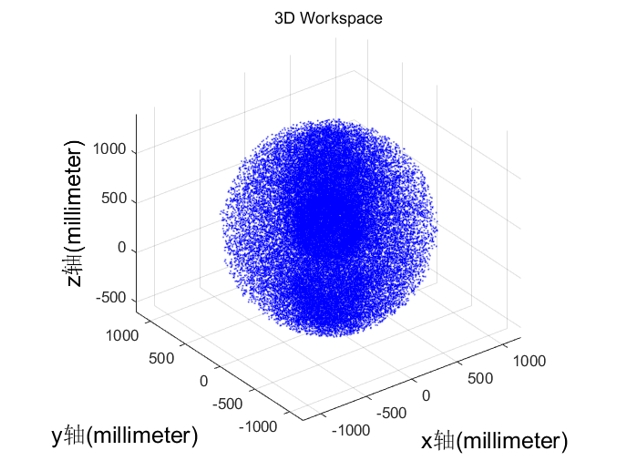
\includegraphics[width=6cm]{Image/fig16.jpg}
    }
    %\caption{fig1}
    \quad
    \subfigure[$N=10^5$]{
    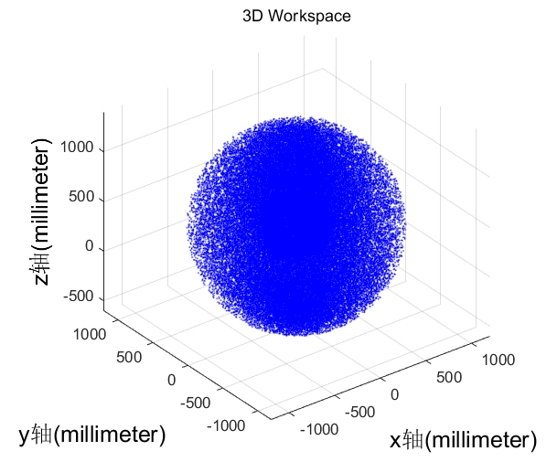
\includegraphics[width=6cm]{Image/fig17.jpg}
    }
    \quad
    \subfigure[$N=5\times 10^5$]{
    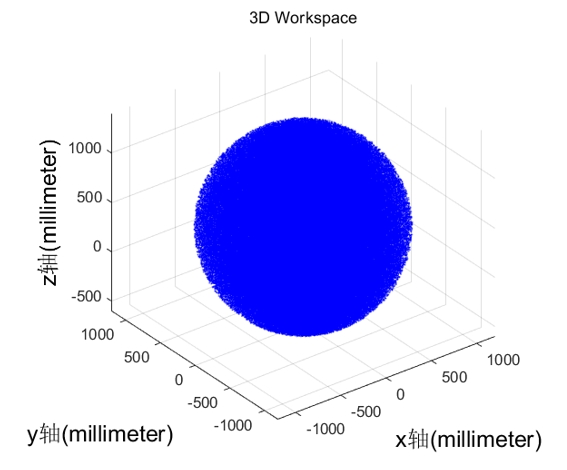
\includegraphics[width=6cm]{Image/fig18.jpg}
    }
    \quad
    \subfigure[$N=10^6$]{
    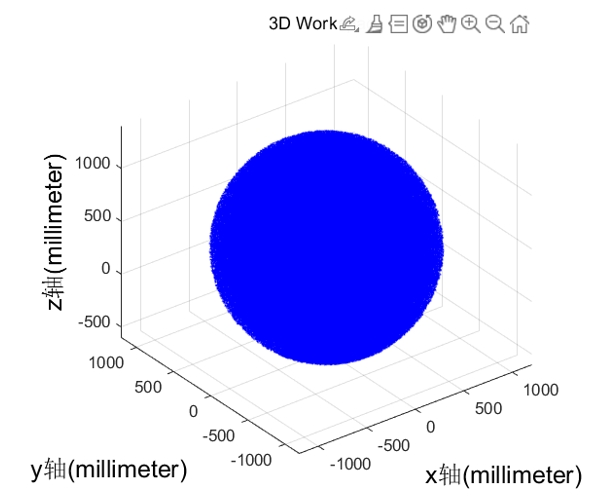
\includegraphics[width=6cm]{Image/fig19.jpg}
    }
    \caption{不同N下工作空间的示意图}
    \label{fig:12}
    \end{figure}


\newpage

%PART II Chapter5-7
\section{数学建模和计算}
\subsection{改进DH参数表}
改进DH参数表(Modified DH,MDH)是一种用于描述机器人机械臂各个关节之间的几何关系的方法。MDH参数表比传统的DH参数表更灵活,可以处理更多类型的机器人结构。基于我们小组的机械臂模型参数,设计MDH如表\ref{tab:4}所示:

\begin{table}[h]
	\centering
    \caption{ABB-IRB-1200模型MDH参数表}
    \label{tab:4}
    \vspace{5pt}
	\setlength{\tabcolsep}{4mm}{
	\begin{tabular}{
	>{\columncolor[HTML]{DAE8FC}}c |
	>{\columncolor[HTML]{DAE8FC}}c |
	>{\columncolor[HTML]{DAE8FC}}c |
	>{\columncolor[HTML]{DAE8FC}}c |
	>{\columncolor[HTML]{DAE8FC}}c |
	>{\columncolor[HTML]{DAE8FC}}c |
	>{\columncolor[HTML]{DAE8FC}}c }
	\hline\hline
	\diagbox{Parameter}{Joints}		 & 1           & 2           & 3             & 4            & 5            & 6            \\ \hline
	$\theta$ & $\theta_1+0$ & $\theta_2+0$ & $\theta_3-90$ & $\theta_4+0$ & $\theta_5+0$ & $\theta_6+0$ \\ \hline
	$d$      & 0.38         & 0           & 0             & 0.34          & 0            & 0.27          \\ \hline
	$\alpha_{i-1}$ & 0           & -90          & 0             & -90          & 90           & -90           \\ \hline
	$a_{i-1}$      & 0           & 0           & 0.35          & 0            & 0            & 0            \\ \hline\hline
	\end{tabular}}
\end{table}

MDH参数表的确定,对后续雅各比矩阵计算、运动学和动力学的计算和仿真等工作都有重要意义。

\subsection{Jacobi矩阵}
机器人雅克比矩阵描述的是关节速度和末端笛卡尔速度和角速度之间的关系。计算雅各比矩阵的常用方法有矢量积法和微分变换法,其中使用矢量积法得到的雅各比矩阵是相对于基坐标系的,微分变换法得到的是相对于末端坐标系的。由于相对于基坐标系的雅各比矩阵比较直接,我们采用矢量积法来求解。

我们所设计的机器人六个关节均为转动关节。而对于转动关节,雅各比矩阵各列元素可以用以下公式表示:

\begin{equation}
    \begin{bmatrix}
        v\\
        w
    \end{bmatrix}=\begin{bmatrix}
        z_i \times ^ip_n^0\\
        z_i
    \end{bmatrix} \dot{q}_i; \quad  J_i =\begin{bmatrix}
        z_i \times ^ip_n^0\\
        z_i
    \end{bmatrix}
\end{equation}

列向量$J_i$表示末端速度、角速度与i关节的角速度之间的关系,将6个列向量组合即可得到机器人的雅各比矩阵,即:
\begin{equation}
    J=\begin{bmatrix}
        J_1 & J_2 & J_3 & J_4 & J_5 & J_6
    \end{bmatrix}
\end{equation}

具体来说,使用矢量积法得到雅各比矩阵需要经过以下步骤,首先根据MDH参数表得到各连杆间的变换矩阵${^{i-1}T}_i$,之后计算各连杆至基坐标系的变换矩阵${^0T}_i$,然后从得到的矩阵中,可以找到$z_i$和$^ip_n^0$的对应元素,最后使用矢量积法公式就可以得到雅各比矩阵了。

根据所设计的机器人的MDH参数表,我们可以利用以下公式计算各连杆间的变换矩阵${^{i-1}T}_i$:
\begin{equation}
    {^{i-1}T}_i=\begin{bmatrix}
        cos \theta_i & -sin \theta_i & 0 & a_{i-1}\\
        sin \theta_i cos \alpha_{i-1} & cos \theta_i cos \alpha_{i-1} & -sin \alpha_{i-1} & -sin \alpha_{i-1}d_i\\
        sin \theta_i sin \alpha_{i-1} & cos \theta_i sin \alpha_{i-1} & cos \alpha_{i-1} & cos \alpha_{i-1}d_i\\
        0 & 0 & 0 & 1
    \end{bmatrix}
\end{equation}

带入各关节的参数,可以得到:
\begin{equation*}
    ^0T_1=\left[ \begin{matrix}	cos\!\:\theta _1&		-sin\!\:\theta _1&		0&		0\\	sin\!\:\theta _1&		cos\!\:\theta _1&		0&		0\\	0&		0&		1&		0.38\\	0&		0&		0&		1\\\end{matrix} \right] \mathrm{      }^1T_2=\left[ \begin{matrix}	cos\!\:\theta _2&		-sin\!\:\theta _2&		0&		0\\	0&		0&		1&		0\\	-sin\!\:\theta _2&		-cos\!\:\theta _2&		0&		0\\	0&		0&		0&		1\\\end{matrix} \right] 
\end{equation*}

\begin{equation*}
    ^2T_3=\left[ \begin{matrix}	sin\!\:\theta _3&		cos\!\:\theta _3&		0&		0.35\\	-cos\!\:\theta _3&		sin\!\:\theta _3&		0&		0\\	0&		0&		1&		0\\	0&		0&		0&		1\\\end{matrix} \right] \mathrm{      }^3T_4=\left[ \begin{matrix}	cos\!\:\theta _4&		-sin\!\:\theta _4&		0&		0\\	0&		0&		1&		0.34\\	-sin\!\:\theta _4&		-cos\!\:\theta _4&		0&		0\\	0&		0&		0&		1\\\end{matrix} \right] 
\end{equation*}

\begin{equation*}
    ^4T_5=\left[ \begin{matrix}	\cos \!\:\theta _5&		-\sin \!\:\theta _5&		0&		0\\	0&		0&		-1&		0\\	\sin \!\:\theta _5&		\cos \!\:\theta _5&		0&		0\\	0&		0&		0&		1\\\end{matrix} \right] \mathrm{      }^5T_6=\left[ \begin{matrix}	cos\!\:\theta _6&		-sin\!\:\theta _6&		0&		0\\	0&		0&		1&		0.27\\	-sin\!\:\theta _6&		-cos\!\:\theta _6&		0&		0\\	0&		0&		0&		1\\\end{matrix} \right] 
\end{equation*}

之后,我们可以计算出各连杆至基坐标系的变换矩阵${^0T}_i$,并从中得到$z_i$和$^ip_n^0$的对应元素,最后使用矢量积法公式就可以得到雅各比矩阵了。

\begin{equation}
    \left\{
        \begin{aligned}
            ^0T_2&=^0T_1 \times ^1T_2\\
            ^0T_3&=^0T_1 \times ^1T_2 \times ^2T_3\\
            ^0T_4&=^0T_1 \times ^1T_2 \times ^2T_3 \times ^3T_4\\
            ^0T_5&=^0T_1 \times ^1T_2 \times ^2T_3 \times ^3T_4 \times ^4T_5\\
            ^0T_6&=^0T_1 \times ^1T_2 \times ^2T_3 \times ^3T_4 \times ^4T_5 \times ^5T_6
        \end{aligned}
    \right.
\end{equation}

$z_i$为3维列向量,其3个元素即为${^0T}_i$第三列的前三个元素。$^ip_n^0$为3维列向量,$^ip_n^0=^6p_0-^ip_0$,其中$^ip_0 $($i$取值范围为1-6)也是3维向量,其3个元素即为${^0T}_i$第四列的前三个元素。

将$z_i$和$^ip_n^0$对应带入矢量积法的公式中,最终可以得到雅各比矩阵。若取初始情况,即$\theta_i=0$($\theta_3$有初始$-90^\circ$的偏置角),结果为:

\begin{equation*}
    J=\begin{bmatrix}
        0 & 0 & 0 & 0 & 0 & 0\\
        0.96 & 0 & 0 & 0 & 0 & 0\\
        0 & -0.96 & -0.61 & 0 & -0.27 & 0\\
        0 & 0 & 0 & 1 & 0 & 1\\
        0 & 1 & 1 & 0 & 1 & 0\\
        1 & 0 & 0 & 0 & 0 & 0
    \end{bmatrix}
\end{equation*}

上述过程可以通过MATLAB代码实现,首先设计计算各连杆间的变换矩阵${^{i-1}T}_i$的函数:

\textbf{Code 1 {\quad} 计算各连杆间的变换矩阵${^{i-1}T}_i$的函数}
\begin{lstlisting}
function T = trans(theta, d, a, alpha)
T = [cos(theta),-sin(theta),0,a;
sin(theta)*cos(alpha), cos(alpha)*cos(theta),-sin(alpha),-d*sin(alpha);
sin(theta)*sin(alpha), sin(alpha)*cos(theta), cos(alpha), d*cos(alpha);
0, 0, 0, 1];
end

\end{lstlisting}

然后将MDH参数带入,求得$^{i-1}T_i$,这里以计算$^5T_6$为例:
\begin{lstlisting}
T56 = trans(theta6, 0.27, 0, -pi/2);   %连杆6至连杆5的变换矩阵
\end{lstlisting}

接着使用矩阵连乘的方法得到各连杆至基坐标系的变换矩阵$^0T_i$,以求$^0T_6$为例:
\begin{lstlisting}
T06 = T01*T12*T23*T34*T45*T56;   %连杆6至基坐标系的变换矩阵
\end{lstlisting}

然后从$^0T_i$中得到$z_i$和$^ip_n^0$的对应元素,带入矢量积法公式中得到$J_i$,以求$J_1$为例:
\begin{lstlisting}
P01 = [T01(1,4);T01(2,4);T01(3,4)];
P06 = [T06(1,4);T06(2,4);T06(3,4)];
z1 = T01(1:3,3);
j1 = [cross(z1,P06-P01);z1];   %矢量积法求J1
\end{lstlisting}

最后,将6个列向量组合得到机器人的雅各比矩阵:
\begin{lstlisting}
Jacobian1 = [j1,j2,j3,j4,j5,j6];   %机器人的雅各比矩阵
\end{lstlisting}

在MATLAB的robotics toolbox库中有求解雅各比矩阵的对应函数,其中jacob0代表相对于基坐标系的雅各比矩阵求解,与我们使用矢量积法得到的结果相同。以下是初始状态下两种方法得到的结果对比,如下图\ref{fig:13}所示:

\begin{figure}[h]
    \centering
    \subfigure[工具包函数jacob0的计算]{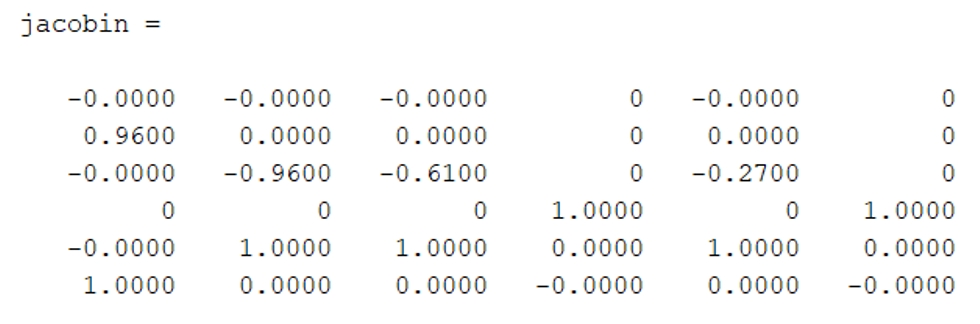
\includegraphics[width=0.4\textwidth]{Image/fig20.jpg}}
    \subfigure[使用矢量积法的雅各比矩阵]{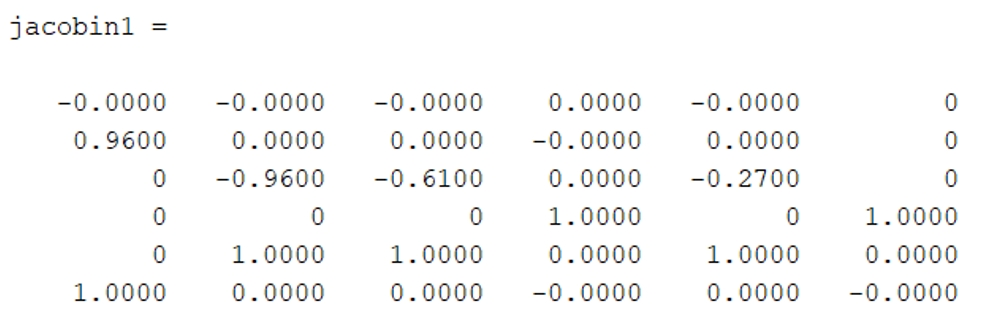
\includegraphics[width=0.4\textwidth]{Image/fig21.jpg}}
    \caption{两种方法得到的雅各比矩阵对比}
    \label{fig:13}
\end{figure}

\subsection{安装方式和自重比计算}
在机械臂设计与应用中,自重负载比是一个关键的参数,它直接影响到机械臂的稳定性和工作效率。在本次研究中,我们考察了不同安装方式对机械臂自重负载比的影响,包括地面安装、墙壁安装与悬挂安装。

首先需要计算各安装方式的最大载荷:我们通过调研和计算,得出了每种安装方式所能承受的最大力。
\begin{enumerate}
    \item \textbf{地面安装}:地面安装方式下,机械臂的自重负载比相对较低,因为地面提供了最大的支撑力。
    \item \textbf{墙壁安装}:机械臂的自重负载比最高。因为墙壁提供的支撑力需要同时承受机械臂自重和操作时的动载荷。
    \item \textbf{悬挂安装}:自重负载比介于地面安装和墙壁安装之间。悬挂安装需要考虑更多的动态因素,如机械臂的摆动和扭矩。
\end{enumerate}

根据上述数据,我们可以计算出各种安装方式的最大载荷,如表\ref{tab:5}所示:

\begin{table}[h]
    \centering
    \caption{不同安装方式的最大载荷}
    \vspace{5pt}
    \label{tab:5}
    \begin{tabular}{
    >{\columncolor[HTML]{ECF4FF}}c 
    >{\columncolor[HTML]{ECF4FF}}c 
    >{\columncolor[HTML]{ECF4FF}}c 
    >{\columncolor[HTML]{ECF4FF}}c }
    \hline \hline
    安装方式   & 力        & 最大载荷(N) & 总最大载荷(N) \\ \hline
    Ground & $F_{xy}$ & 1620    & 2284     \\ \hline
    Ground & $F_z$    & 1610    & /        \\ \hline
    Wall   & $F_{xy}$ & 1940    & 2358     \\ \hline
    Wall   & $F_z$    & 1340    & /        \\ \hline
    Hang   & $F_{xy}$ & 1620    & 2284     \\ \hline
    Hang   & $F_z$    & 1610    & /        \\ \hline \hline
    \end{tabular}
    \end{table}

接下来我们进行了力的示意与分析工作:我们使用了力的示意图来分析不同安装方式下机械臂受力的情况。图\ref{fig:14}与图\ref{fig:15}展示了机械臂在不同安装方式下的受力方向和力的分布情况。

\begin{figure}[htbp]
    \centering
    \subfigure[受力前视图]{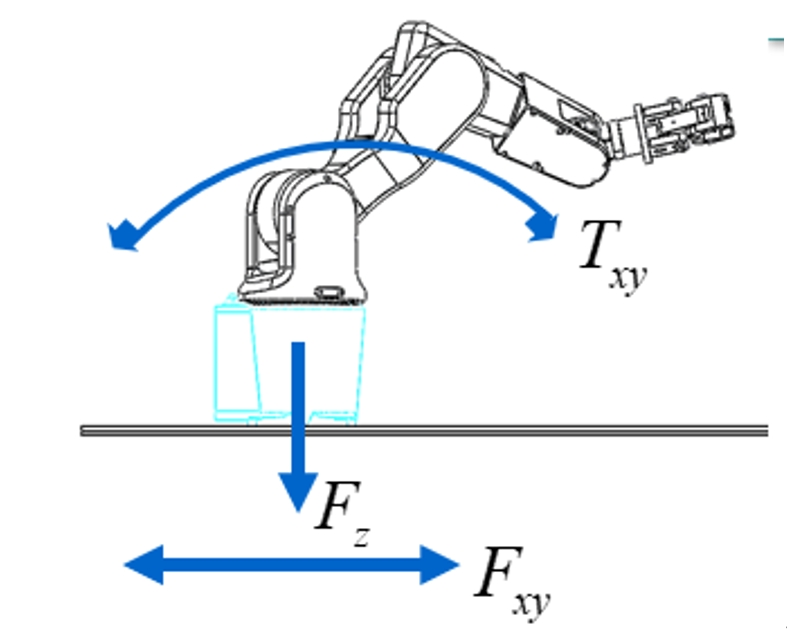
\includegraphics[width=0.4\textwidth]{Image/fig23.jpg}
    \label{fig:14}}
    \subfigure[受力上视图]{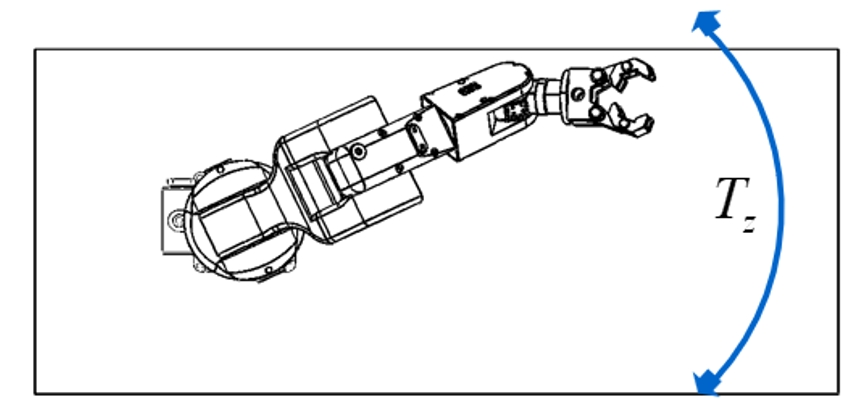
\includegraphics[width=0.4\textwidth]{Image/fig24.jpg}
    \label{fig:15}}
    \caption{机械臂受力示意图}
\end{figure}

最终我们得到最大自重负载比:

在机械臂自重52kg的条件下,我们得出最大自重负载比出现在墙壁安装方式下,最大自重负载比为:
\begin{equation*}
    \frac{2358}{52 \times 9.8}=4.53
\end{equation*}

该值表明在墙壁安装情况下,机械臂能够承受的最大载荷为其自重的4.53倍。墙壁安装方式能够在保持稳定性的前提下,承受较大的操作载荷。

我们对上述过程进行了分析,得出以下结论:
\begin{itemize}
    \item 装方式对自重负载比的影响显著:墙壁安装方式虽然提供了最高的自重负载比,但需要在设计时充分考虑安装结构的强度和稳定性。
    \item 优化设计的重要性:为了在实际应用中实现最佳性能,需要根据具体的使用环境和操作要求,选择合适的安装方式,并对机械臂的设计进行优化。
\end{itemize}


\section{运动学计算和实现}
\subsection{正向运动学}
正向运动学描述了从机器人关节空间到末端执行器位置和姿态的变换。具体来说,正向运动学计算的是给定关节变量(如关节角度或关节位移)时,末端执行器在工作空间中的位置和方向。

根据MDH参数表,我们在5.2小节已经计算得到了各连杆间的变换矩阵,我们据此可以计算得到末端位姿:
$$
    ^0T_6=^0T_1 \times ^1T_2 \times ^2T_3 \times ^3T_4 \times ^4T_5 \times ^5T_6=
$$
\begin{figure}[htbp]
    \centering
    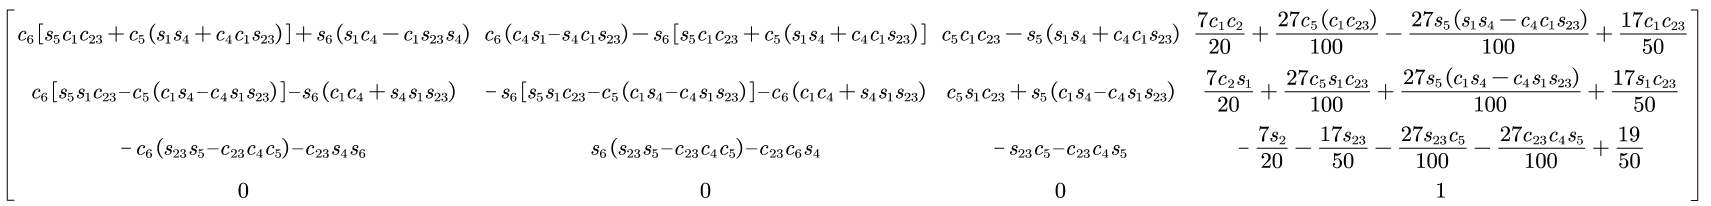
\includegraphics[width=\textwidth]{Image/fig25.jpg}
\end{figure}

其中$s_i=sin\theta_i,c_i=cos\theta_i,s_{ij}=sin\left(\theta_i+\theta_j\right),c_{ij}=cos\left(\theta_i+\theta_j\right)$。

即实现了正向运动学——根据各关节角度信息计算得到末端位姿信息.

\subsection{逆向运动学}
机器人的逆运动学共有8组解,以下为求解过程。

设$\boldsymbol{p}_w$为4坐标系原点在基坐标系的坐标。

设输入矩阵为:
\begin{equation}
    T_{6}^{0}=\left[ \begin{matrix}	R_{6}^{0}&		p_{6}^{0}\\	0&		1\\\end{matrix} \right] 
\end{equation}

通过末端位姿反推到
\begin{equation}
    p_w=p_{6}^{0}-R_{6}^{0}\left[ \begin{array}{c}	0\\	0\\	0.27\\\end{array} \right] =\left[ \begin{array}{c}	p_{wx}\\	p_{wy}\\	p_{wz}\\\end{array} \right] 
\end{equation}

正向运算:
\begin{equation}
    T_{3}^{0}=\left[ \begin{matrix}	c_1s_{23}&		c_1c_{23}&		-s_1&		\frac{7c_1c_2}{20}\\	s_1s_{23}&		s_1c_{23}&		c_1&		\frac{7s_1c_2}{20}\\	c_{23}&		-s_{23}&		0&		\frac{19}{50}-\frac{7s_2}{20}\\	0&		0&		0&		1\\\end{matrix} \right]
\end{equation}

\begin{equation}
    \left[ \begin{array}{c}	p_{wx}\\	p_{wy}\\	p_{wz}\\	1\\\end{array} \right] =T_{3}^{0}\left[ \begin{array}{c}	0\\	0.34\\	0\\	1\\\end{array} \right] =\left[ \begin{array}{c}	\frac{7c_1c_2}{20}+\frac{17c_1c_{23}}{50}\\	\frac{7s_1c_2}{20}+\frac{17s_1c_{23}}{50}\\	\frac{19}{50}-\frac{7s_2}{20}-\frac{17s_{23}}{50}\\	1\\\end{array} \right] 
\end{equation}

得到方程:
\begin{equation}
    \left\{ \begin{array}{c}	\mathrm{    }\frac{7}{20}c_1c_2+\frac{17}{50}c_1c_{23}=p_{wx}\\	\mathrm{    }\frac{7}{20}s_1c_2+\frac{17}{50}s_1c_{23}=p_{wy}\mathrm{ }\\	\mathrm{    }\frac{7}{20}s_2+\frac{17}{50}s_{23}=-p_{wz}+\frac{19}{50}\\\end{array} \right.
\end{equation}

前两个等式做线性变换可得:
\begin{equation}
    \left\{ \begin{array}{c}	\mathrm{    }p_{wx}s_1=p_{wy}c_1\\	\mathrm{    \theta}_1=Atan2\left( p_{wy},p_{wx} \right) +\frac{\mathrm{\pi}}{2}\pm \frac{\mathrm{\pi}}{2}\\\end{array} \right. 
\end{equation}

注意此处有2个解。

\begin{enumerate}
    \item 当$p_{wx} \neq 0$时,将$\theta_1$代入方程组得到
    \begin{equation}
        \left\{ \begin{array}{c}	\frac{7}{20}c_2+\frac{17}{50}c_{23}=\frac{p_{wx}}{c_1}\\	\frac{7}{20}s_2+\frac{17}{50}s_{23}=-p_{wz}+\frac{19}{50}\\\end{array} \right. 
    \end{equation}


两边同时平方后相加,得到:
\begin{equation}
    c_3=\frac{500}{119}\left( \frac{p_{wx}^{2}}{c_{1}^{2}}+p_{wz}^{2}-\frac{19}{25}p_{wz}-\frac{937}{10000} \right) 
\end{equation}

于是

\begin{equation}
    \begin{aligned}
        \theta_3&=arccos\left[ \frac{500}{119}\left( \frac{p_{wx}^{2}}{c_{1}^{2}}+p_{wz}^{2}-\frac{19}{25}p_{wz}-\frac{937}{10000} \right) \right] +\frac{\mathrm{\pi}}{2}\pm \frac{\mathrm{\pi}}{2}\\
        &=arccos\left[ \frac{500}{119}\left( p_{wx}^2+p_{wy}^2+p_{wz}^{2}-\frac{19}{25}p_{wz}-\frac{937}{10000} \right) \right] +\frac{\mathrm{\pi}}{2}\pm \frac{\mathrm{\pi}}{2}
    \end{aligned}
\end{equation}

    \item 当$p_{wx}=0$时,有
    \begin{equation}
        \left\{ \begin{array}{c}	\mathrm{    }\frac{7}{20}c_2+\frac{17}{50}c_{23}=p_{wy}\\	\frac{7}{20}s_2+\frac{17}{50}s_{23}=-p_{wz}+\frac{19}{50}\\\end{array} \right.
    \end{equation}

    同理可以得到:
    \begin{equation}
        \mathrm{\theta}_3=arccos\left[ \frac{500}{119}\left( p_{wy}^{2}+p_{wz}^{2}-\frac{19}{25}p_{wz}-\frac{937}{10000} \right) \right] +\frac{\mathrm{\pi}}{2}\pm \frac{\mathrm{\pi}}{2}
    \end{equation}

\end{enumerate}
    综合上述两种情况,我们可以得到$\theta_3$的两个解:
    \begin{equation}
        \mathrm{\theta}_3=arccos\left[ \frac{500}{119}\left( p_{wx}^{2}+p_{wy}^{2}+p_{wz}^{2}-\frac{19}{25}p_{wz}-\frac{937}{10000} \right) \right] +\frac{\mathrm{\pi}}{2}\pm \frac{\mathrm{\pi}}{2}
    \end{equation}

    当$\left( p_{wz}-\frac{19}{50} \right) ^2+p_{wx}^{2}+p_{wy}^{2}\neq 0$时,解得:

    \begin{equation}
        \begin{aligned}
            c_2 &=\frac{\left( \frac{7}{20}+\frac{17}{50}c_3 \right) \sqrt{p_{wx}^{2}+p_{wy}^{2}}-\frac{17}{50}s_3\left( p_{wz}-\frac{19}{50} \right)}{\left( p_{wz}-\frac{19}{50} \right) ^2+p_{wx}^{2}+p_{wy}^{2}}\\
            s_2 &=-\frac{\left( \frac{7}{20}+\frac{17}{50}c_3 \right) \left( p_{wz}-\frac{19}{50} \right) +\frac{17}{50}s_3\sqrt{p_{wx}^{2}+p_{wy}^{2}}}{\left( p_{wz}-\frac{19}{50} \right) ^2+p_{wx}^{2}+p_{wy}^{2}}
        \end{aligned}
    \end{equation}

    因此有$\theta_2 = Atan2(s_2,c_2)$,在$\theta_3$确定的条件下,$\theta_2$唯一,故$(\theta_1,\theta_2,\theta_3)$共有4组解。

    \textcolor{cherry}{特殊情况:}当$\left( p_{wz}-\frac{19}{50} \right) ^2+p_{wx}^{2}+p_{wy}^{2} = 0$时,\textbf{无解}。

接下来求解$\theta_4,\theta_5,\theta_6$,我们可以得到:
\begin{equation}
    \begin{aligned}
        R_{3}^{0}&=\left[ \begin{matrix}	\mathrm{c}_1\mathrm{s}_{23}&		\mathrm{c}_1\mathrm{c}_{23}&		-\mathrm{s}_1\\	\mathrm{s}_1\mathrm{s}_{23}&		\mathrm{s}_1\mathrm{c}_{23}&		\mathrm{c}_1\\	\mathrm{c}_{23}&		-\mathrm{s}_{23}&		0\\\end{matrix} \right] \\
        R_{6}^{3}&=\left( R_{3}^{0} \right) ^{-1}R_{6}^{0}=\left[ \begin{matrix}	n_x&		s_x&		a_x\\	n_y&		s_y&		a_y\\	n_z&		s_z&		a_z\\\end{matrix} \right] 
    \end{aligned}
\end{equation}

可得到4组$R_6^3$。又:
\begin{equation}
    \begin{aligned}
        &R_{6}^{3}=R_{4}^{3}R_{5}^{4}R_{6}^{5}=\left[ \begin{matrix}	c_4c_5c_6-s_4s_6&		-s_4c_6-c_4c_5s_6&		-c_4s_5\\	s_5c_6&		-s_5s_6&		c_5\\	-s_4c_6-s_4c_5c_6&		s_4c_5s_6-c_4c_6&		s_4s_5\\\end{matrix} \right] \\
        &\left[ \begin{matrix}	c_4c_5c_6-s_4s_6&		-s_4c_6-c_4c_5s_6&		-c_4s_5\\	s_5c_6&		-s_5s_6&		c_5\\	-s_4c_6-s_4c_5c_6&		s_4c_5s_6-c_4c_6&		s_4s_5\\\end{matrix} \right] =\left[ \begin{matrix}	n_x&		s_x&		a_x\\	n_y&		s_y&		a_y\\	n_z&		s_z&		a_z\\\end{matrix} \right]
    \end{aligned}  
\end{equation}

首先$c_5=a_y$,故$s_5=\pm\sqrt{1-a_y^2}$,共有两组解.

\begin{enumerate}
    \item $s_5=\sqrt{1-a_y^2}$ 时:
    
    \begin{equation}
        \begin{aligned}
            &\mathrm{\theta}_4=Atan2\left( \frac{a_z}{\sqrt{1-a_{y}^{2}}},-\frac{a_x}{\sqrt{1-a_{y}^{2}}} \right)\\
            & \mathrm{\theta}_5=Atan2\left( \sqrt{1-a_{y}^{2}},a_y \right) \\
            & \mathrm{\theta}_6=Atan2\left( -\frac{s_y}{\sqrt{1-a_{y}^{2}}},\frac{n_y}{\sqrt{1-a_{y}^{2}}} \right)
        \end{aligned}
    \end{equation}

    \item $s_5=-\sqrt{1-a_y^2}$ 时:
    
    \begin{equation}
        \begin{aligned}
            \mathrm{\theta}_4&=Atan2\left( -\frac{a_z}{\sqrt{1-a_{y}^{2}}},\frac{a_x}{\sqrt{1-a_{y}^{2}}} \right)\\
            \mathrm{\theta}_5&=Atan2\left( -\sqrt{1-a_{y}^{2}},a_y \right)\\
            \mathrm{\theta}_6&=Atan2\left( \frac{s_y}{\sqrt{1-a_{y}^{2}}},-\frac{n_y}{\sqrt{1-a_{y}^{2}}} \right) 
        \end{aligned}
    \end{equation}
\end{enumerate}

综上所述,我们可以得到机器人的逆运动学解,共有8组解。

为验证运算结果是否正确,项目组设计了配套于该机器人的函数ikine8(T)。以机器人的末端位姿作为输入,函数可输出8组逆运动学解。经验证,我们使用ikine8(T)得到的解集中有一组解与使用robotics工具包自带函数ikine(T)得到的解相同。

事实上,在进行机器人运动轨迹规划时,会得到包含大量组逆运动学解的集合,此时将选取随时间变化连续的逆解,使机器人可以平滑地运动,不出现瞬移,代码细节在附件-运动学代码中给出。

\subsection{运动学功能拓展实现}
基于运动学正逆解,我们为机械臂设计了两个特殊功能,末端画出圆形轨迹和空中截物检测。具体功能描述和展示如下:

\subsubsection{末端圆形轨迹绘制}
功能描述:输入圆心、半径、圆法向旋转矩阵,生成相应圆作为机器人末端轨迹,使用运动学逆解输出旋转角组绘制动画。

\textbf{Code 2 {\quad} 末端圆形轨迹绘制函数}
\begin{lstlisting}
DrawCircle(Centre, Radius, Face);
\end{lstlisting}

其形式参数——Centre:圆心 Radius:半径 Face:法向旋转矩阵。通过三个关键参数,我们可以绘制出机械臂末端的圆形轨迹,效果如图\ref{fig:16}所示,具体代码实现在附件-运动学代码中给出。

\begin{figure}[htbp]
    \centering
    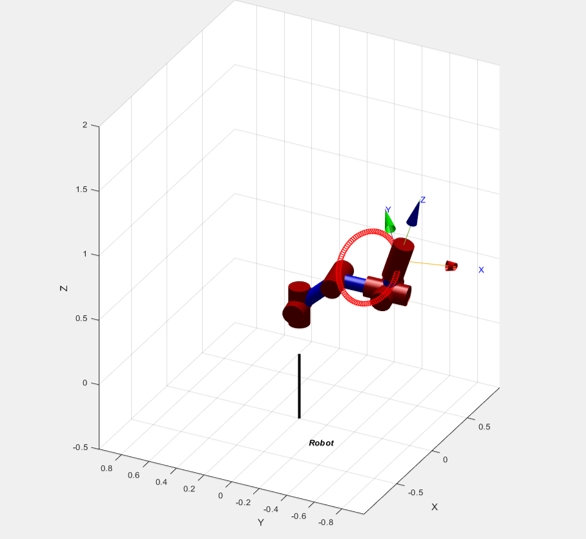
\includegraphics[width=0.6\textwidth]{Image/fig26.jpg}
    \caption{DrawCircle()函数末端圆形轨迹绘制效果}
    \label{fig:16}
\end{figure}
\subsubsection{空中截物检测}
\textbf{功能描述:}输入初始末端位姿T0;两个物体的初始位置P1、P2;初速度V1、V2;接物总时间$t_m$;中途接物后摇$t_s$;接到物体时规定末端位姿R1、R2(默认为$\left[\begin{matrix}0&0&1\\0&-1&0\\1&0&0\\\end{matrix}\right]$),输出机器人轨迹对应的旋转角解集组。

\textbf{原理分析}:设物体的初始位置为$P_{i0}$,初速度为$V_i$,加速度$A=\left[\begin{matrix}0\\-g\\0\\\end{matrix}\right]$。

于是$P=\int_{0}^{t}\left(V_i+A\tau\right)d\tau=P_{i0}+V_it+\frac{1}{2}At^2$,代入$ t$ 可得到任意时刻物体位置。

由于样条插值得到的轨迹为曲线,为减少计算量,仅考虑直线距离以规划接物顺序与时间。

代入$t_m$得到两物终点$P_{1m}$、$P2m$。机器人末端初始位置$P_0$已知。调整接中间物的时间$ t_c$使$\frac{\mid P\left(t_c\right)-P_0\mid}{\mid P_m-P\left(t_c\right)\mid}$ 最接近$\frac{t_c}{t_m-t_c}$ ,将此情况视为最优。更改先后顺序,选取两组最优轨迹总距离最小者。

\textbf{Code 3 {\quad} 空中截物检测函数}
\begin{lstlisting}
CatchBall(T0,P1,P2,V1,V2,tm,ts,R1,R2)
\end{lstlisting}

形式参数——T0:初始末端位姿 ;P1,P2:物体初始位置 ;
V1,V2:物体初速度; tm:接物限时 ;
ts:接物间隔  ;    R1,R2:接物时刻末端旋转矩阵。


\textbf{仿真展示}:如图\ref{fig:17}所示。左图为接到第一个物体时两物轨迹和机器人位姿,右图为接到第二个物体时两物轨迹(此时第一个物体的轨迹已停止继续生成)和机器人位姿。

\begin{figure}[htbp]
    \centering
    \subfigure[Situation 1]{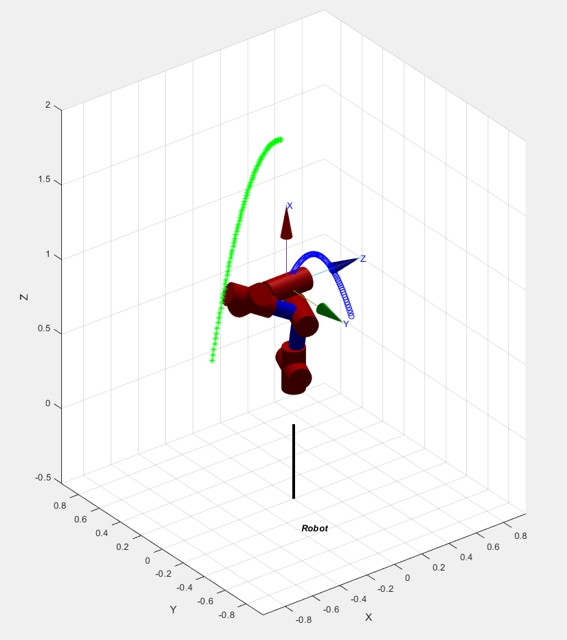
\includegraphics[width=0.4\textwidth]{Image/fig27.jpg}}
    \subfigure[Situation 2]{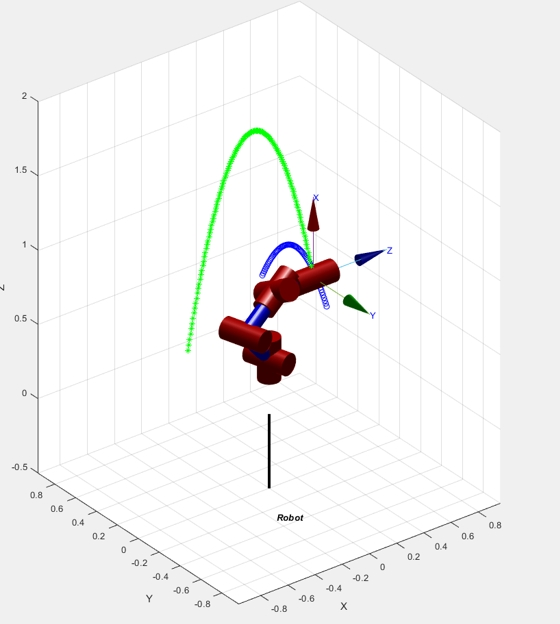
\includegraphics[width=0.4\textwidth]{Image/fig28.jpg}}
    \caption{空中截物检测仿真展示}
    \label{fig:17}
\end{figure}

如果我们是用\textbf{面向对象编程}的思想,我们可以将机器人的运动学功能封装成一个类MYROBOT,则可以通过我们写的这两个函数来实现机器人的运动学的特殊功能\verb|MYROBOT.DrawCircle();MYROBOT.CatchBall();|,用户并不需要了解具体的运动学原理,只需要调用这两个函数即可实现,这也很好的契合了我们一直以来所强调的工程思想。

\newpage
\section{动力学计算和实现}
\subsection{Lagrange方程求解}
构建拉格朗日方程分析机器人的动力学——首先,拉格朗日函数为$ L=T-U$,其中T为系统动能,U为系统势能。
则n自由度系统的拉格朗日方程可以表示为:
\begin{equation}
    \frac{d}{dt}\left( \frac{\partial L}{\partial \dot{q}_i} \right) - \frac{\partial L}{\partial q_i} = \tau_i ; \quad i=1,2,...,n
\end{equation}

其中,$q_i$为系统的广义坐标,$\tau_i$为广义坐标对应的广义力。

现在分别对连杆$L_i$的动能、势能进行计算,最后带入到拉格朗日方程中求解。为了简化计算,我们使用等效质心的方式表示连杆,且电机和连杆壳体不分开计算,记为同一整体。

\textbf{首先是对连杆$L_i$的动能计算}:

假设连杆$L_i$的质量为$m_i$,在基坐标系下连杆$L_i$的质心向量$p_i=\frac{1}{m_i}\int_{0}^{V_i}{p_i^\ast\rho dV}$,其中$p_i^\ast$为连杆$L_i$上任意一点的坐标。令$r_i=p_i^\ast-p_i$,则$p_i^\ast$的速度为:

\begin{equation}
    \dot{p_i^{\ast}} = \dot{p_i} + \omega_i \times r_i = \dot{p_i} + S(\omega_i)r_i
\end{equation}

进而,我们可以对连杆$L_i$上每一个点$p_i^\ast$的动能进行积分,得到连杆$L_i$的位移动能和转动动能分别为:
\begin{equation}
    \left\{ \begin{array}{c}	\mathrm{    }T_t=\frac{1}{2}m_i\dot{p_i}^T\dot{p_i}\\	\mathrm{    }T_r=\frac{1}{2}{\omega _i}^TI_i\omega _i=\frac{1}{2}{\omega _i}^T[R_{i}^{0} \cdot I_{i}^{i} \cdot \left( R_{i}^{0} \right) ^T]\omega _i\\\end{array} \right.
\end{equation}

其中,$I_i$代表基坐标系下$L_i$的转动惯量矩阵,$I_i^i$代表$L_i$坐标系下下$L_i$的转动惯量矩阵,二者之间存在关系$I_i=R_i^0 I_i^i (R_i^0)^T$.

则连杆$L_i$的动能可以表示为:
\begin{equation}
    T_i=\frac{1}{2}m_i\dot{p_i^T}\dot{p_i}+\frac{1}{2}\omega_i^T[R_i^0I_i^i(R_i^0)^T]\omega_i
\end{equation}

其中,$\dot{p_i}=J_{P1}^i\dot{q_1}+ \cdots +J_{Pi}^i\dot{q_i}=J_P^i\dot{q}$,$\omega_i=J_{o1}^i\dot{q_1}+\cdots +J_{oi}^i\dot{q_i}=J_o^i\dot{q}
$。\\

由于本机器人6个关节均为转动关节,对于转动关节有:
\begin{equation}
    \begin{cases}
        J_{pi}=z_i^0\times (p_e^0-p_i^0)\\
        J_{oi}=z_i^0
    \end{cases}
\end{equation}

代入动能表达式可得连杆$L_i$的动能最终表示为: 
\begin{equation}
    T_i=\frac{1}{2}m_i\dot{q_T}(J_p^i)^TJ_P^i\dot{q}+\frac{1}{2}\dot{q_T}(J_o^i)^T[R_i^0I_i^i(R_i^0)^T]=J_o^i\dot{q}
\end{equation}

由公式可见,给定各杆件质量参数、质心位置参数、转动惯量矩阵和DH参数表,即可计算某种运动轨迹下的连杆动能变化。

\textbf{然后对连杆\(L_i\)的势能计算:}

假设连杆$L_i$的质量为$m_i$,在基坐标系下连杆$L_i$的质心向量为$p_i$,则连杆$L_i$可以表示为:
\begin{equation}
    U_i=-m_ig_0^TP_i
\end{equation}

其中,$g_0=[0\quad 0\quad -g]^T$。由公式可见,给定各杆件质量参数、质心位置参数和DH参数表,即可计算某
种运动轨迹下的连杆势能变化。

\textbf{把上述结果带入到拉格朗日方程计算和化简:}

机器人系统总动能、总势能为各杆件之和(不考虑负载的情况)。即:
\[
T=\sum_{i=1}^{6}T_i\quad U=\sum_{i=1}^{6}U_i\quad L=T-U
\]

令$B(q)=\sum_{i=1}^{6}m_i(J_p^i)^T J_p^i+(J_o^i)^T[R_i^0I_i^i(R_i^0)^T]J_o^i$,动能T可以由该正定对称矩阵表示为:
\begin{equation}
    T=\frac{1}{2}\dot{q}^TB(q)\dot{q}=\frac{1}{2}\sum_{i=1}^6\sum_{j=1}^6b_{ij}(q)\dot{q_i}\dot{q_j}
\end{equation}

对于坐标$q_i$,有:
\begin{equation}
    \frac{\partial L}{\partial \dot{q_i}}=\frac{\partial T}{\partial \dot{q_i}}=\sum_{j=1}^6b_{ij}(q)\dot{q_j}
\end{equation}

再对t求导,得到拉格朗日方程第一项:
\begin{equation}
    \frac{d}{dt}\frac{\partial L}{\partial\dot{q_i}}=\sum_{j=1}^6b_{ij}\ddot{q_j}+\sum_{i=1}^6\sum_{j=1}^6\frac{\partial b_{ij}(q)}{\partial q_k}\dot{q_k}\dot{q_j}
\end{equation}

再求拉格朗日方程的第二项:
\begin{equation}
    \frac{\partial T}{\partial \dot{q_i}}=\frac{1}{2}\sum_{i=1}^6\sum_{j=1}^6\frac{\partial b_{ij}(q)}{\partial q_k}\dot{q_k}\dot{q_j}
\end{equation}

\begin{equation}
    \frac{\partial U}{\partial q_i}=-\sum_{j=1}^6m_ig_0^T\frac{\partial p_i}{\partial q_i}=g_i(q)
\end{equation}

则有:
\begin{equation}
    \frac{\partial L}{\partial\dot{q_i}}= \frac{\partial T}{\partial \dot{q_i}}- \frac{\partial U}{\partial q_i}=\frac{1}{2}\sum_{i=1}^6\sum_{j=1}^6\frac{\partial b_{ij}(q)}{\partial q_k}\dot{q_k}\dot{q_j}-g_i(q)
\end{equation}


把两项分别带入,可以将拉格朗日方程求解为: 
\begin{equation}
    \sum_{j=1}^6b_{ij}\ddot{q_j}+\frac{1}{2}\sum_{i=1}^6\sum_{j=1}^6\frac{\partial b_{ij}(q)}{\partial q_k}\dot{q_k}\dot{q_j}+g_i(q)=\tau_i
\end{equation}

给定各杆件质量参数、质心位置参数、转动惯量矩阵和DH参数表,用关节转角表示广义坐标:在已知连杆所受广义力的受力情况,可以通过正动力学得到各关节角速度、角加速度;也可以在已知各关节角速度、角加速度,通过逆动力学反解连杆受力情况。 

由拉格朗日方程可见,进行动力学求解,需要设定以下参数:各连杆质量、各连杆质心位置、各连杆转动惯量矩阵、MDH参数表。如以下代码所示: 
设计机器人各关节动力学参数(质量(kg)、质心位置(m)、电机惯性、惯量矩阵($kg*m^2$))\\

\textbf{Code 4 \quad 机器人各关节动力学参数设定}
\begin{lstlisting}
L(1).m=5.235; 
L(1).r=[0.115,0,0.192]; 
L(1).Jm=0.0002; 
L(1).I=10^(-6)*[233372.299 12.446 115929.582; 
            12.446 314433.958 -1424.735; 
            115929.582 -1424.735 104166.070]; 
\end{lstlisting}

其中,质量、质心位置、转动惯量矩阵可以由SolidWorks的“质量属性”功能得到。由于在建模的时候已经考虑了连杆选用的材料,电机选型和安装位置,所测得的参数结果与实际情况已经比较接近;但由于建模时未考虑电线质量等因素,测定结果依然存在些许误差,如下图\ref{fig:99}所示。

\begin{figure}
    \centering
    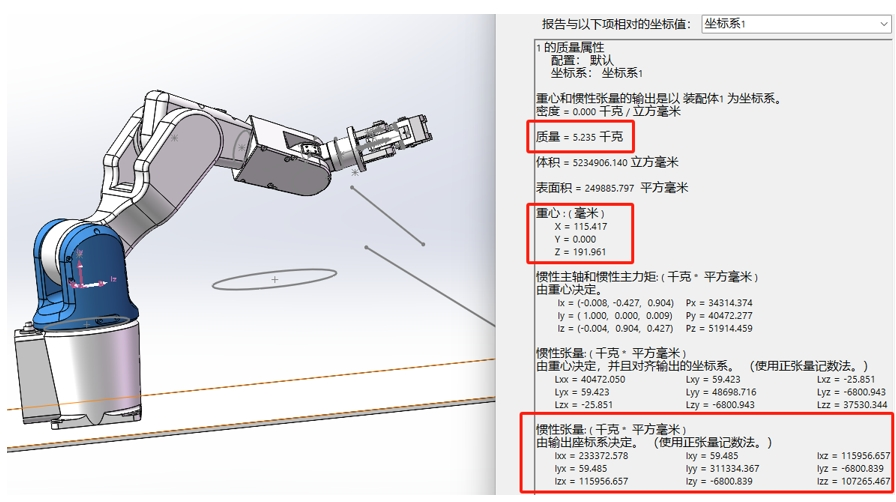
\includegraphics[width=0.8\textwidth]{Image/fig99.png}
    \caption{机器人各关节动力学参数设定}
    \label{fig:99}
\end{figure}
值得一提的是,使用robotics toolbox自带函数“fdyn”进行动力学求解时需要设定电机惯性参数,机器人常用的电机惯性参数为$10^{-4}$左右。电机惯性参数对计算结果影响不大。 

\newpage
\subsection{正向动力学}
正向动力学是已知各关节受力/力矩情况,求解关节角、角速度、角加速度等信息。在代码实现时主要用到两个函数,\verb|fdyn()|函数可以给定力矩函数得到关节角、角速度,\verb|accel()|函数可以进一步得到关节角速度,细节如下表\ref{tab:fdyn}所示。

\begin{table}[htbp]
    \centering
    \caption{正向动力学函数}
    \label{tab:fdyn}
    \vspace{5pt}
    \begin{tabular}{ccc}
    \rowcolor[HTML]{5B9BD5} 
    函数                            & 输入参数                  & 输出结果                      \\
    \rowcolor[HTML]{BDD6EE} 
    \cellcolor[HTML]{5B9BD5}\verb|fdyn()|  & 时间范围最大值、力矩函数          & \makecell[c]{时间点序列、每个时间点对应\\的关节角、关节角速度序列} \\
    \rowcolor[HTML]{DEEAF6} 
    \cellcolor[HTML]{5B9BD5}\verb|accel()| & \makecell[c]{时间点序列以及\\对应的关节角、关节角速度序列} & 关节角速度序列                  
    \end{tabular}
\end{table}

以下是代码示例,设定时间为2s之内,$@$ my\_torque\_function为自定义的力矩函数,q1是得到的关节角序列,qd1是得到的关节角速度序列,qdd1是得到的关节角加速度序列,三者与时间点序列t1的各时间点一一对应。

\textbf{Code 5 \quad 正向动力学求解示例}
\begin{lstlisting}
%求解关节角和角速度
[t1,q1,qd1] = robot.nofriction().fdyn(2, @my_torque_function);   
%求解关节角加速度
qdd1 = robot.accel(q1,qd1,tau1);        
\end{lstlisting}

例如,给定$@$my\_torque\_function为常力矩函数,给定各关节力矩如图\ref{fig:torque}所示.

\begin{figure}[htbp]
    \centering
    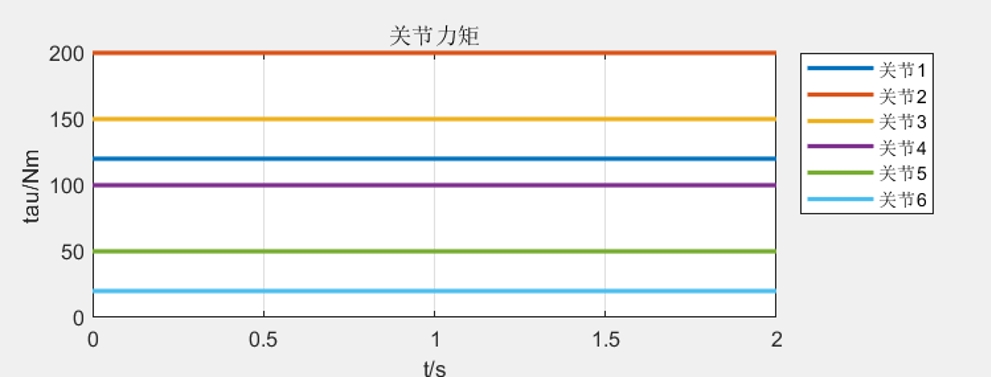
\includegraphics[width=0.8\textwidth]{Image/fig51.png}
    \caption{关节力矩示意图}
    \label{fig:torque}
\end{figure}

使用\verb|fdyn|函数和\verb|accel|函数,得到q1,qd1,qdd1,分别作q1-t1,qd1-t1,qdd-t1图像,即得到关节角、角速度、角加速度随时间变化曲线,如图\ref{fig:q1qd1qdd1}所示。

\begin{figure}[htbp]
    \centering
    \subfigure[关节角随时间变化曲线]{
    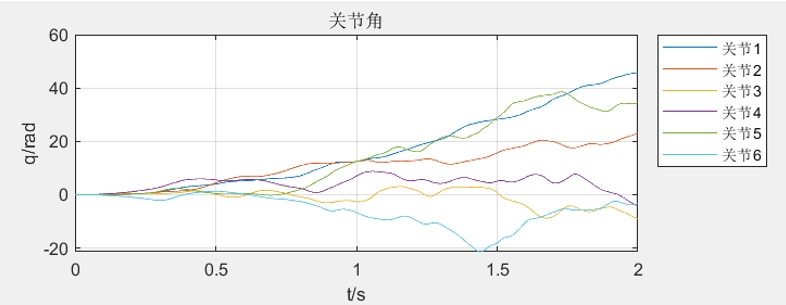
\includegraphics[width=10cm]{Image/fig52.png}
    }
    \subfigure[关节角速度随时间变化曲线]{
    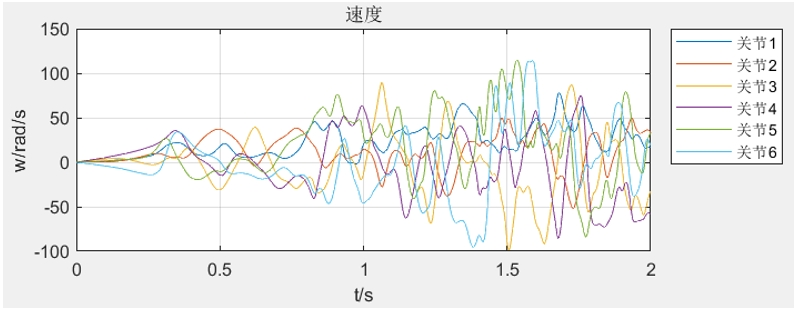
\includegraphics[width=10cm]{Image/fig53.png}
    }
    \subfigure[关节角加速度随时间变化曲线]{
    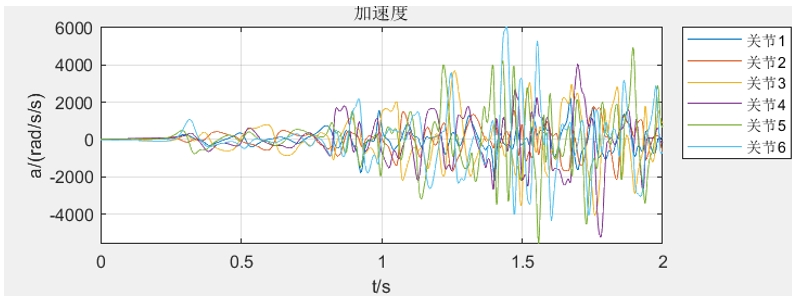
\includegraphics[width=10cm]{Image/fig54.png}
    }
    \caption{关节角、角速度、角加速度随时间变化曲线}
    \label{fig:q1qd1qdd1}
\end{figure}

值得一提的是,robotics toolbox工具包中的fdyn函数底层代码使用的是牛顿-欧拉法,即基于经典力学中的牛顿运动定律和欧拉转动定律推导得出动力学求解结果。这种算法更适合串联式机器人结构,与拉格朗日法相比,牛顿-欧拉法更加直观,但是计算复杂,且难以处理并联式机器人。
\newpage
\subsection{逆向动力学}
逆向运动学是已知各关节角、角速度、角加速度信息,求解各关节受力/力矩情况。在代码实现过程中主要应用\verb|rne()|函数,该函数给定关节角等信息可以得到力矩。关节角等对应参数可以通过运动学的求解得到,细节如下表\ref{tab:rne}所示。

\begin{table}[htbp]
    \centering
    \caption{逆向动力学函数}
    \label{tab:rne}
    \vspace{5pt}
    \begin{tabular}{ccc}
    \rowcolor[HTML]{5B9BD5} 
    函数                            & 输入参数                  & 输出结果                      \\
    \rowcolor[HTML]{BDD6EE} 
    \cellcolor[HTML]{5B9BD5}\verb|rne()|  & \makecell[c]{关节角序列、角速度序列、角加速度序列、\\重力加速度向量(可选,默认为[0 0 9.81])}          &  力矩序列\\                
    \end{tabular}
\end{table}

以下是代码示例,所给定的关节角序列q,角速度序列qd,角加速度序列qdd必须是行数相等的列向量,计算得到的力矩序列tau的行数也与它们相同。例如,给定初始关节角位姿和结束时关节角位姿,用五次多项式法规划得到两个位置之间的移动轨迹,使用逆向运动学的方法求解,得到对应时间点的各关节角、角速度、角加速度序列。

\begin{figure}[htbp]
    \centering
    \subfigure[关节末端轨迹图]{
    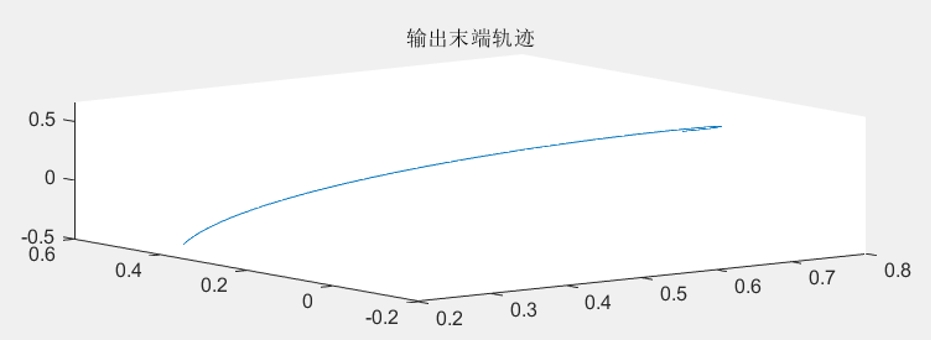
\includegraphics[width=0.4\textwidth]{Image/fig55.png}
    \label{fig:55}
    }
    \subfigure[关节角随时间变化曲线]{
    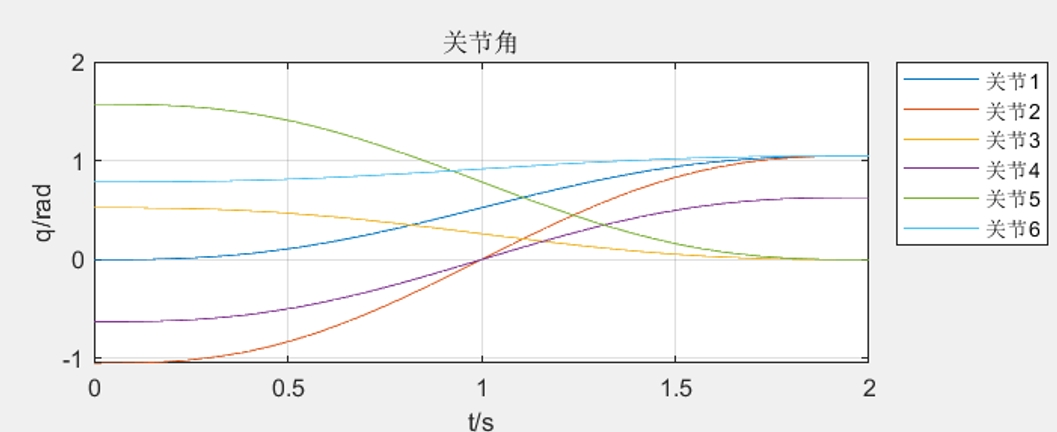
\includegraphics[width=0.4\textwidth]{Image/fig56.png}
    \label{fig:56}
    }
    \subfigure[关节角速度随时间变化曲线]{
    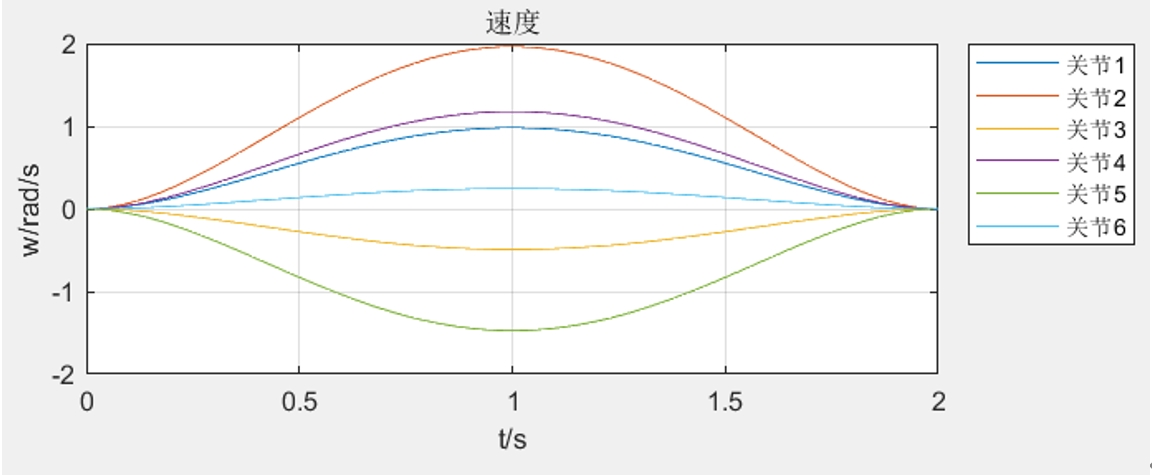
\includegraphics[width=0.4\textwidth]{Image/fig57.png}
    \label{fig:57}
    }
    \subfigure[关节角加速度随时间变化曲线]{
    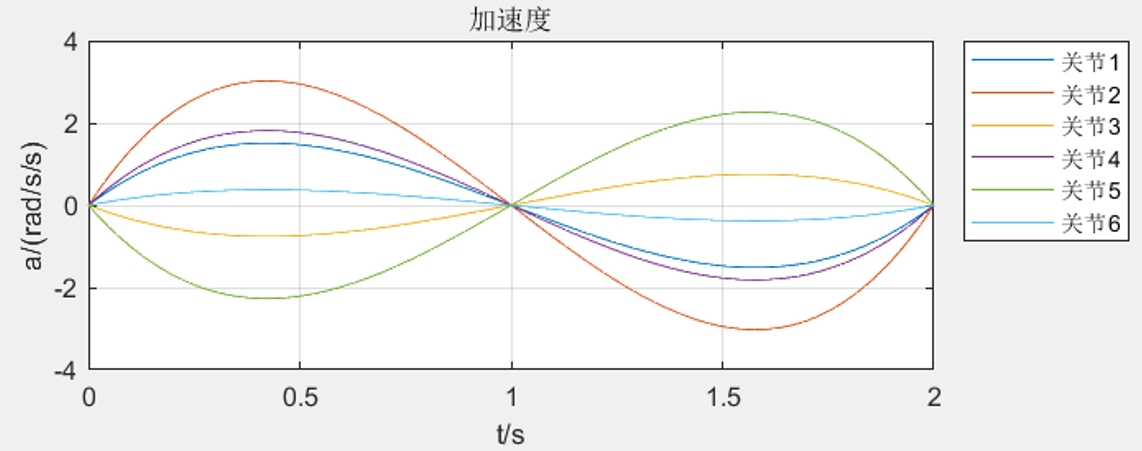
\includegraphics[width=0.4\textwidth]{Image/fig58.png}
    \label{fig:58}
    }
    \caption{逆向动力学求解结果}
\end{figure}

\newpage
\textbf{Code 6 \quad 逆向动力学求解示例}
\begin{lstlisting}
tau=robot.rne(q,qd,qdd,[0 0 9.81]);   
%逆向动力学,根据关节角、角速度、角加速度求解关节力矩,取g=9.81m/s^2
init=[0 -pi/3 pi/6 -pi/5 pi/2 pi/4];   %位置1关节角
targ=[pi/3 pi/3 0 pi/5 0 pi/3];   %位置2关节角
time=0:0.01:2;   %时间序列
%五次多项式规划位置1到位置2的运动轨迹,得到关节角度,角速度,角加速度
[q, qd, qdd]=jtraj(init,targ,time);
\end{lstlisting}   

将上述运行结果绘制成图像,得到关节末端轨迹图、关节角随时间变化曲线、关节角速度随时间变化曲线、关节角加速度随时间变化曲线,如图\ref{fig:55}、\ref{fig:56}、\ref{fig:57}、\ref{fig:58}所示。

将得到的q、qd、qdd带入rne函数中,可以得到力矩序列tau,作tau-time图像,即得到力矩随时间变化曲线。如图\ref{fig:59}所示。

\begin{figure}[htbp]
    \centering
    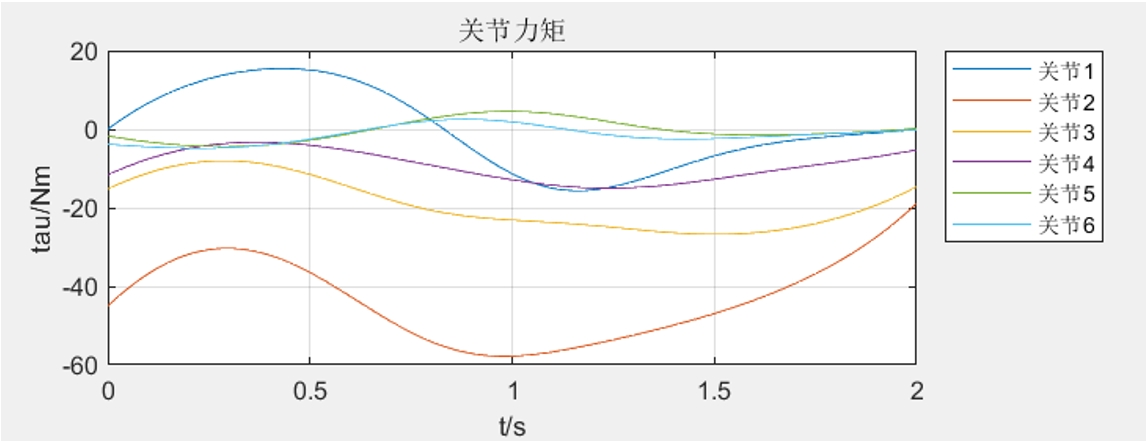
\includegraphics[width=0.8\textwidth]{Image/fig59.png}
    \caption{力矩随时间变化曲线}
    \label{fig:59}
\end{figure}

\newpage

% PART IV Chapter8
\section{运动控制与仿真}
机器人关节控制是指对机器人的各个关节进行精确定位和运动控制,使机器人能够完成各种任务的过程。在先前的部分,我们小组已经对ABB-IRB-1200型号的机器人进行了一个较为逼真的建模和设计,这一部分我们将讨论在虚拟环境中对其进行运动仿真和控制,以期获得我们课程所学内容的一些复现(无论是课程ME3403《机器人学》,还是ME2232《系统模型、分析与控制(A类)》,甚至是一些不是我们学院开设的课程,比如《运动控制系统》等),同时我们也希望能通过这个大作业加深我们对机器人控制科学的认识,补足在课程内由于课时原因造成的一些“不知所学”的现象。

我们想分为3个部分对这个问题进行探讨:
\begin{enumerate}
    \item \textbf{运动学的规划仿真}:这一部分主要是对我们机器人的MDH建系、旋转矩阵的变换、关节操作空间等概念有一个认知,在脱离MATLAB工具包的情况下自行对我们建立的模型进行运动控制和仿真。
    \item \textbf{动力学的控制和仿真I}:这一部分主要研究当输入为一个力矩而不是一个运动时,机器人的相关响应。以及如果我们提供一个信号,如何让机器人进行一个更加优秀的跟踪响应。
    \item \textbf{动力学的控制和仿真II}:这一部分以理论为主,我们将电机抽象成一个一阶系统模型,通过控制框图对机器人单关节的优化控制方法进行了一些调研和复现,这部分以展示为主。
\end{enumerate}

\begin{figure}[htbp]
    \centering
    
\includegraphics[width=0.8\textwidth]{Image/logo.png}
    \caption{本大作业使用的仿真软件支持}
    \label{fig:18}
\end{figure}

我们主要使用了Solidworks和MATLAB联合仿真,如图\ref{fig:18}。在“军火展示”之前,我们写了一个配置文件\textcolor{cherry}{Configuration.pdf}(附在作业提交的压缩包中),这份文件作为我们大作业的辅助项目,介绍了如何通过Solidworks + MATLAB/Simulink和Simscape/Multibody进行联合仿真。这份指导文件中还说明了我们的一些信号(比如梯形速度曲线Trapezoidal-Curve和S型速度曲线S-Curve)在Simulink中如何生成。

导入XML文件后,可以看到图\ref{fig:19}所示的页面。通过Simulink中加入一些信号模块等作为输入,可以指导我们对运动进行仿真。

\begin{figure}[htbp]
    \centering
    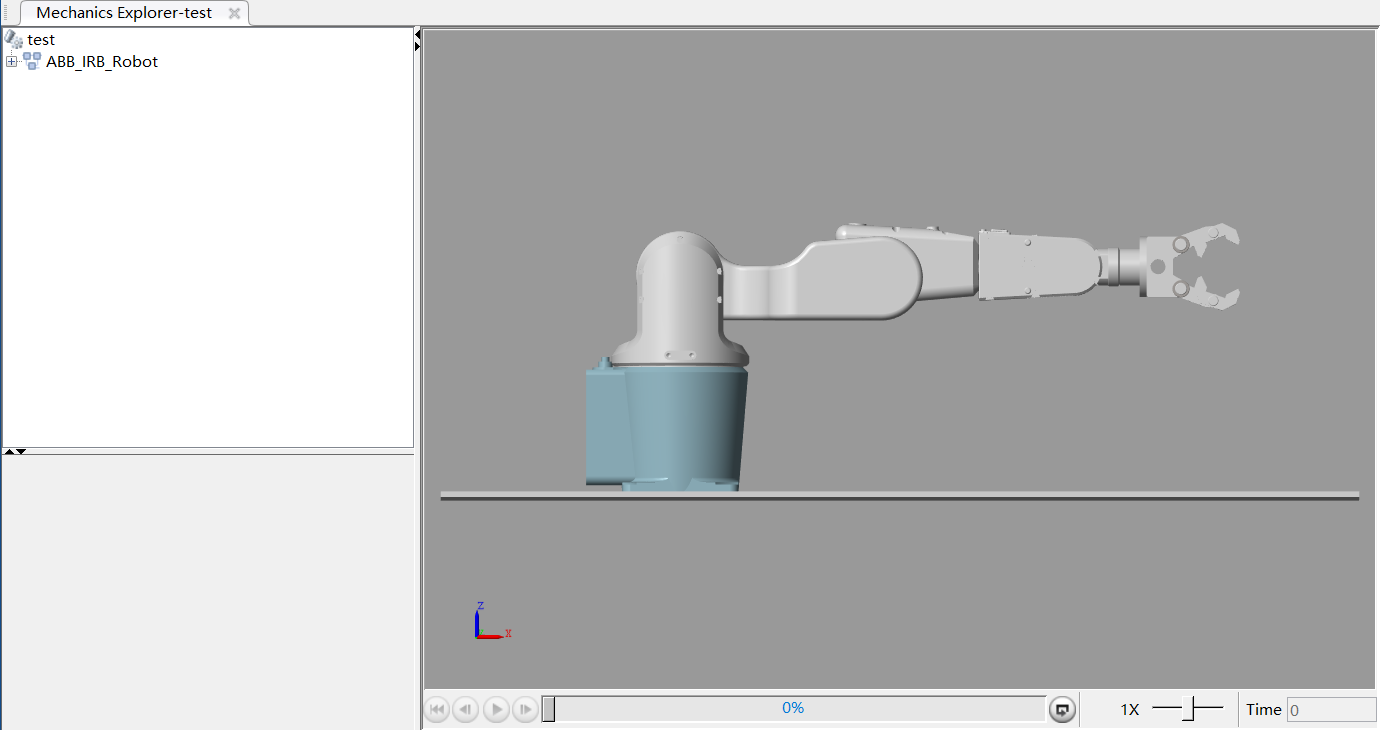
\includegraphics[width=0.8\textwidth]{Image/initial.png}
    \caption{我们小组建模的ABB-IRB-1200机器人在Simulink中的仿真页面}
    \label{fig:19}
\end{figure}

在Simulink中,一个六自由度机器人的模块化框图如下图37所示,其主要的模块有3个:Solid(刚体)、Rigid Transform (刚体坐标变换)、Revolute Joint(旋转关节)。具体的配置在文件中有说明。我们还在旋转关节中设置了传感器,反馈关节的速度、位置等信息,对应现实生活中的速度传感器和位移传感器(绝对值编码器)。

\begin{figure}[htbp]
    \centering
    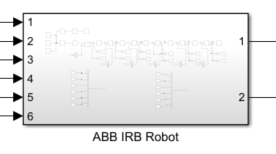
\includegraphics[width=0.4\textwidth]{Image/ABBsubsys.png}
    \caption{将机器人模型整合为6输入2输出的子系统}
    \label{fig:21}
\end{figure}

具体的模型结构如图\ref{fig:20}所示。

\begin{figure}[htbp]
    \centering
    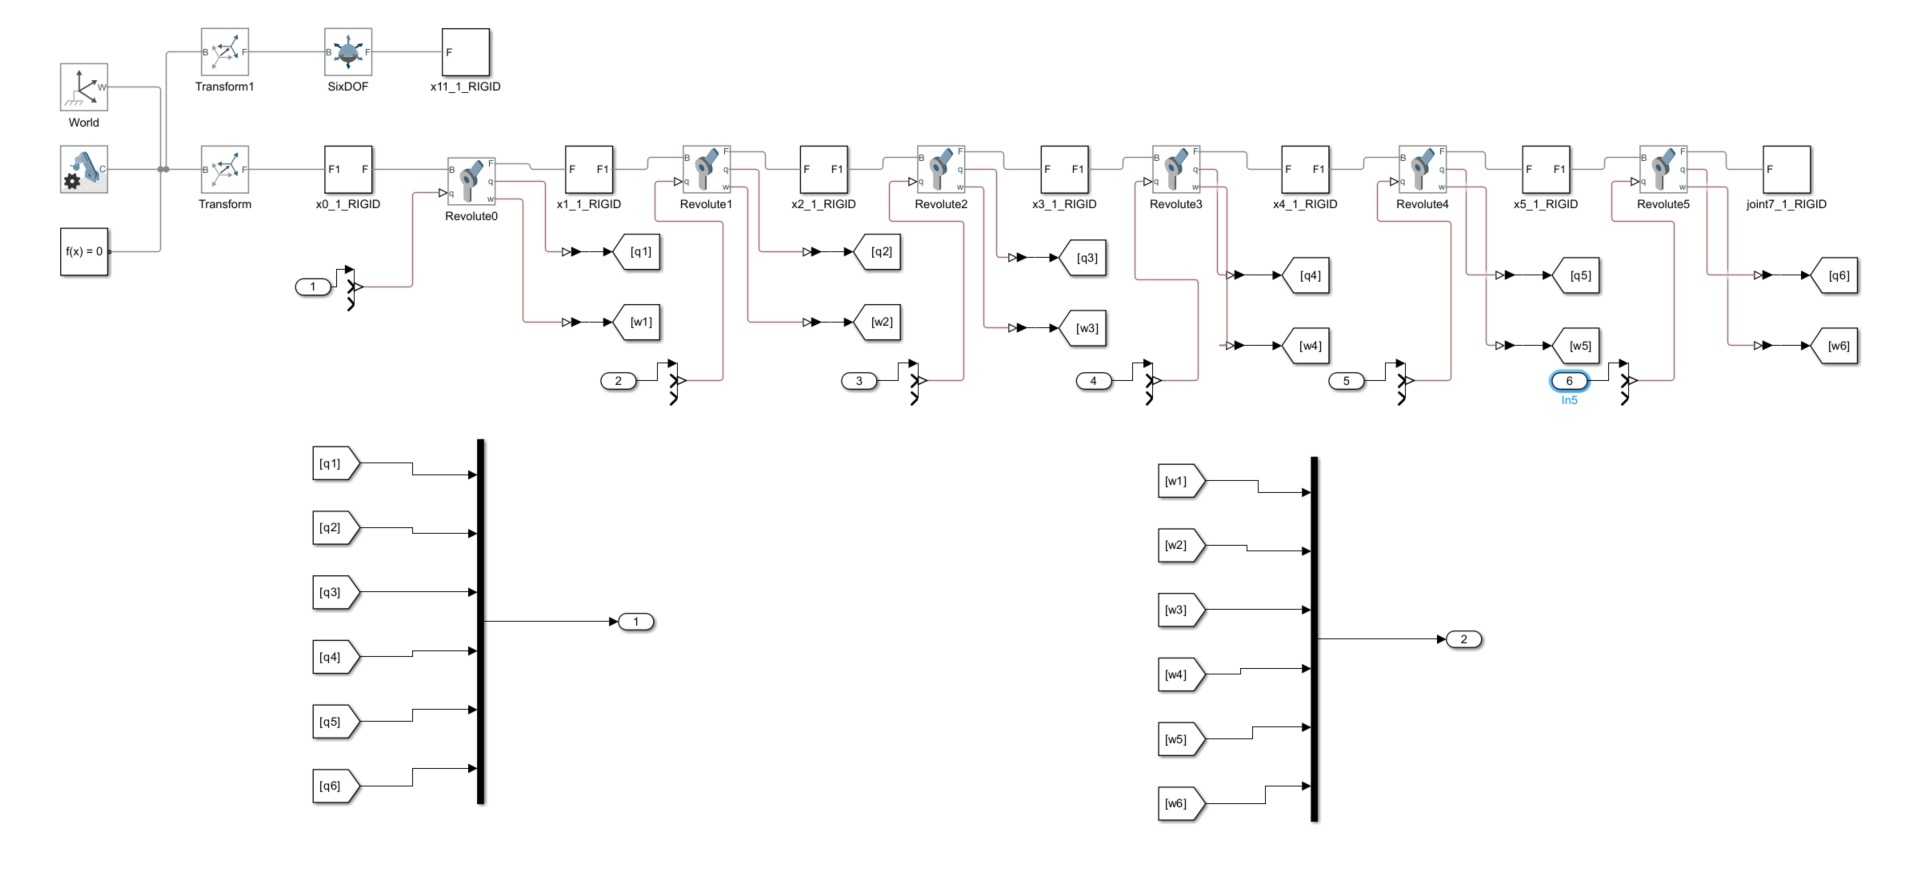
\includegraphics[width=0.7\textwidth]{Image/ABBIRB.png}
    \caption{ABB-IRB-1200机器人在Simulink中的模型结构}
    \label{fig:20}
\end{figure}

将其输入、输出通过“Mux”整合,建立一个子系统,方便面向对象的仿真操作(即我们的用户并不需要知道机器人内部的配置)。这样我们可以更好地将“面向对象”的思想纳入大作业的使用,提高我们的工程学素养,如图\ref{fig:21}所示。



\subsection{基于模型的运动学仿真}
我们将Solidworks模型导入Simscape后,把Revolute Joint的输出调节为运动信号输入模式“q”。这样的结果是模型中展示关节的运动角(直接体现运动)。如下图\ref{fig:22}所示,其余的参数比如初始角、刚度、阻尼等可以通过实际情况提供的参数进行修改。在Simulink中搭建的模型如图\ref{fig:23}所示。

\begin{figure}[htbp]
    \centering
    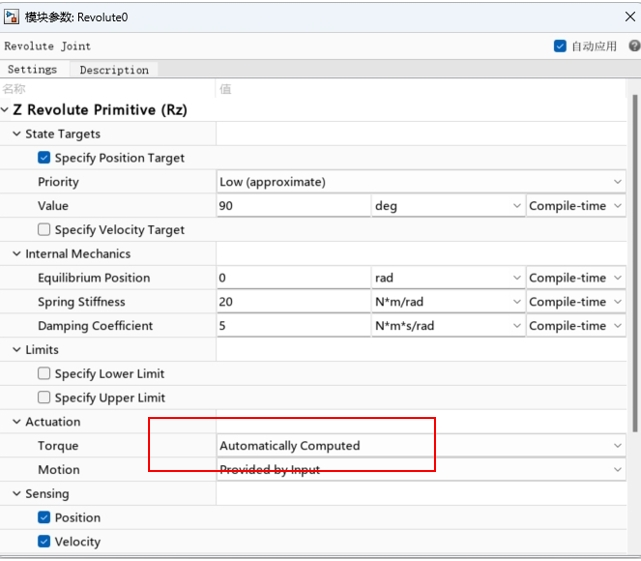
\includegraphics[width=0.4\textwidth]{Image/motion.png}
    \caption{关节运动输入模式}
    \label{fig:22}
\end{figure}

\begin{figure}[htbp]
    \centering
    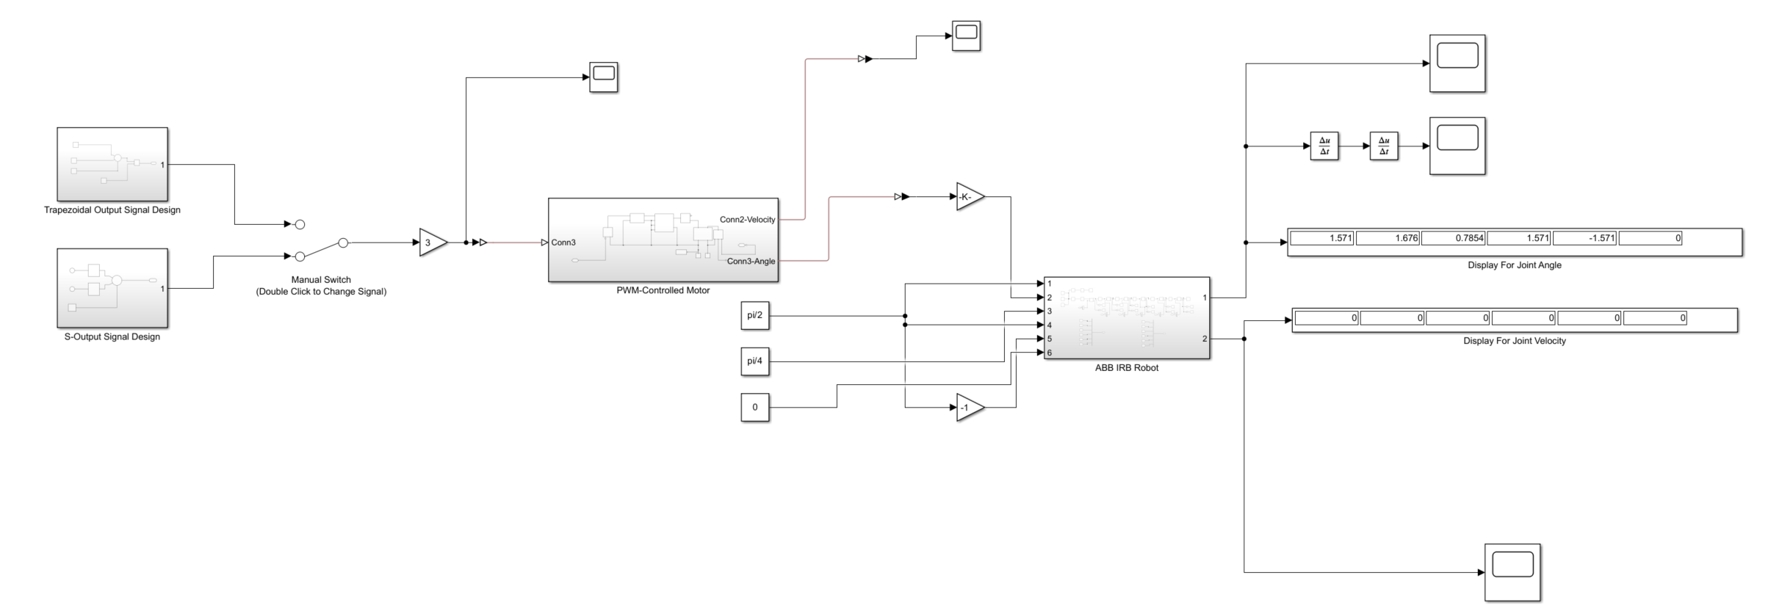
\includegraphics[width=0.8\textwidth]{Image/sim-motion.png}
    \caption{关节运动仿真模型}
    \label{fig:23}
\end{figure}

考察一个转动关节(2\#,大臂回旋),我们采用梯形运动信号输入和S型运动信号输入对机器人的运动进行模拟,可以得到关于梯形信号和S型信号的运动动画。由于报告中不方便插入视频,且转换为GIF格式后清晰度下降影响观感,因此这部分的动画可以参考附件视频或者PPT中对应的页码(Page40-Trapezoidal Signal,42-S Signal)。

\begin{figure}[htbp]
    \centering
    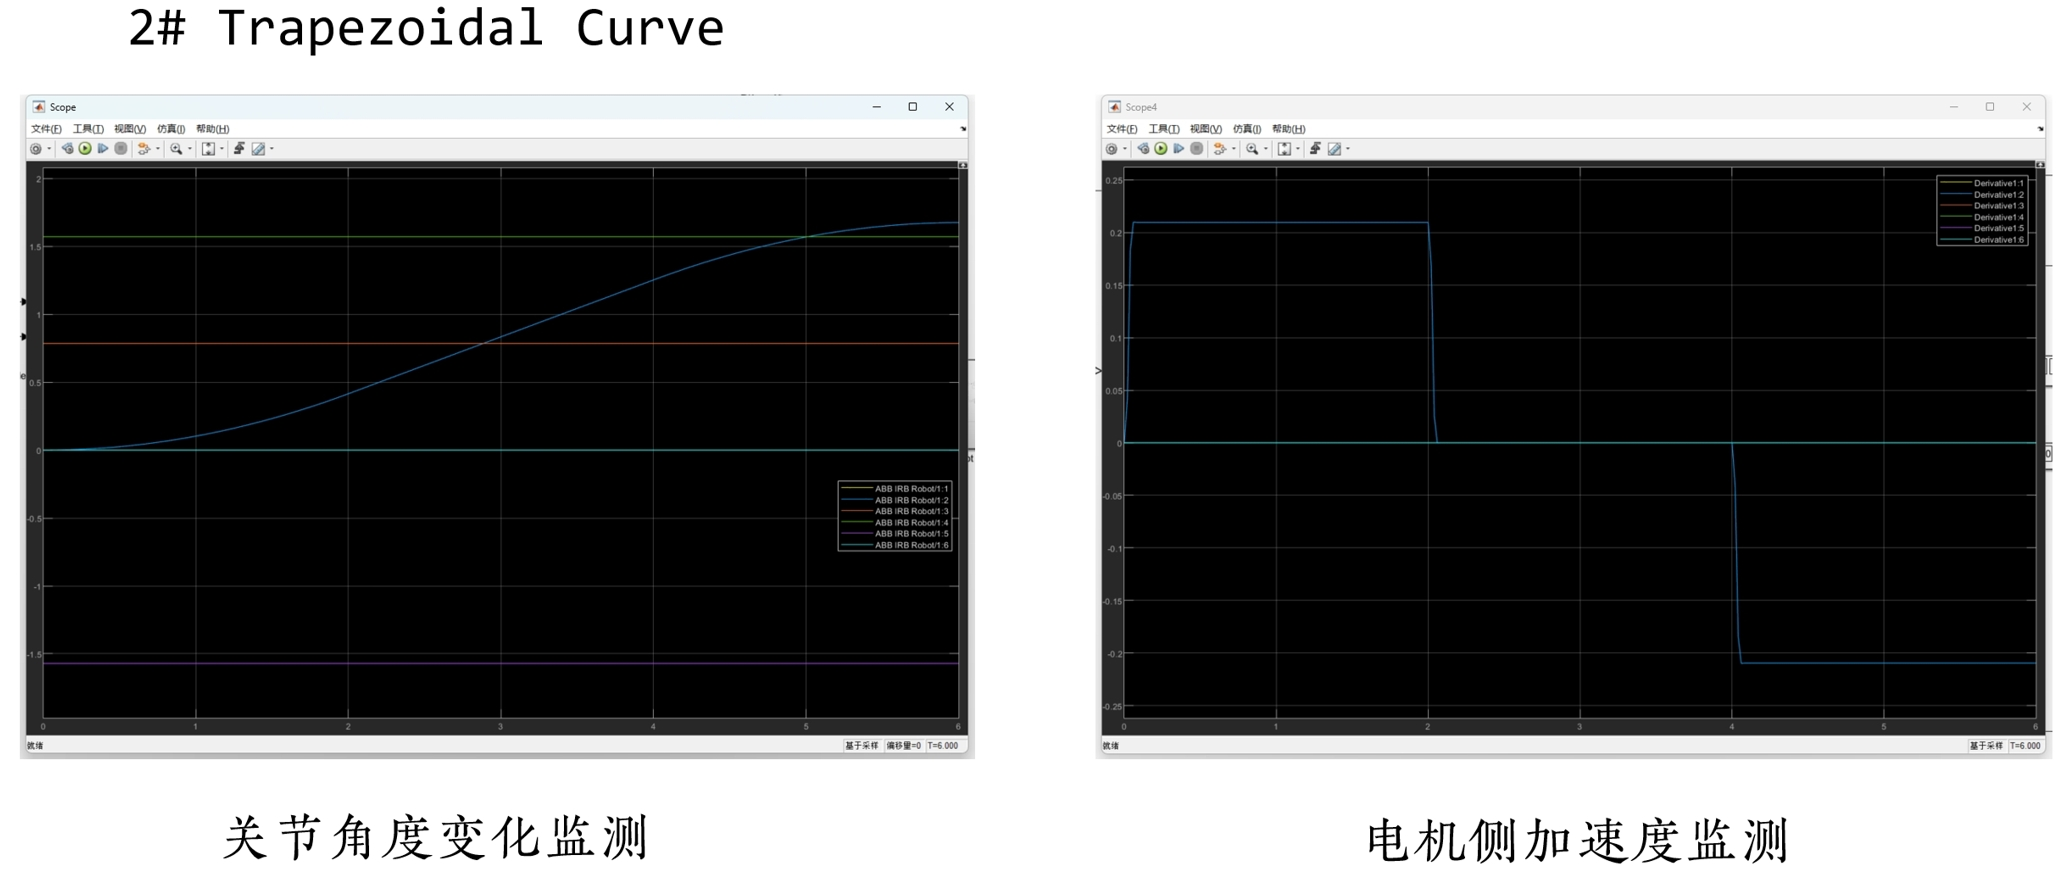
\includegraphics[width=\textwidth]{Image/fig30.png}
    \caption{梯形速度曲线下关节角度和电机侧加速度}
    \label{fig:24}
\end{figure}

对于这两种信号的应用在工程界也是有所讲究的。在工程界的电机控制中,梯形速度曲线和S型速度曲线的应用主要是为了优化电机的性能和保护机械系统。梯形速度曲线因其简单性和易于实现,广泛用于需要较快响应和精确定位的场合。这种速度曲线由加速、匀速和减速三个阶段组成,使得电机能够快速加速到目标速度,并在目标位置准确停止。然而,梯形速度曲线的加速度变化较为突兀(如图\ref{fig:24}所示),在实际的工程过程中由于工件的刚性可能会引起机械系统的振动和冲击,从而导致磨损和噪音。


相比之下,S型速度曲线则通过逐渐变化的加速度来平滑速度变化,如图\ref{fig:25}所示。显著减少了机械系统的冲击和振动。S型速度曲线的平滑过渡使其非常适合于需要高平稳性的应用,如精密加工和高精度运动控制场合,尽管其实现相对复杂且计算量较大。因此在梯形速度曲线和S型速度曲线的选择中,应用和需求通常要权衡。实际机器人的响应速度、定位精度以及系统的机械负载和寿命都是重要的考察因素。

\begin{figure}[htbp]
    \centering
    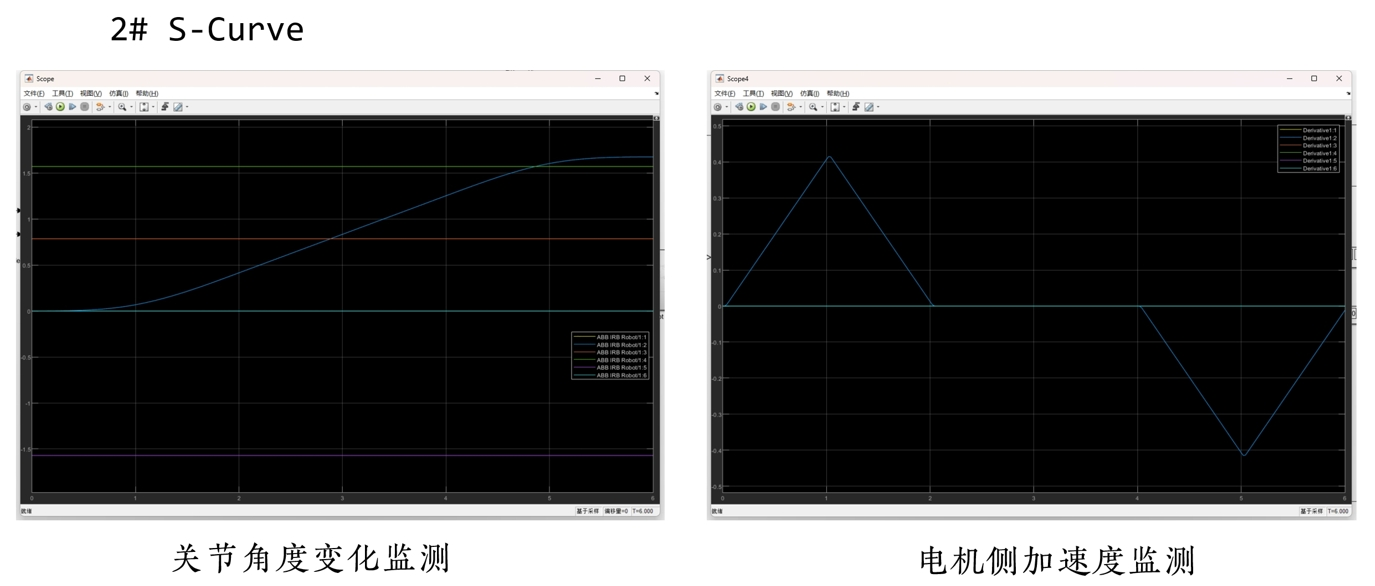
\includegraphics[width=\textwidth]{Image/fig31.png}
    \caption{S型速度曲线下关节角度和电机侧加速度}
    \label{fig:25}
\end{figure}

当然,我们也可以用一些诸如正弦、阶跃等常规的模块来构造信号观察运动,还可以采用自己设计的信号。在前面提到的运动学计算里,我们可以通过DrawCircle(Center, Radius, Face)函数来设计一个空间中的平面圆。通过求解并定义运动点数(比如200)我们能得到函数返回值q矩阵(200*6)。通过Simulink的“From Workspace”模块导入数据,并在左侧增广一个时间序列t(200*1),即可做出相应的运动(运动过程视频参见PPT或附件),机器人各关节角度如图\ref{fig:26}所示。

\begin{figure}[htbp]
    \centering
    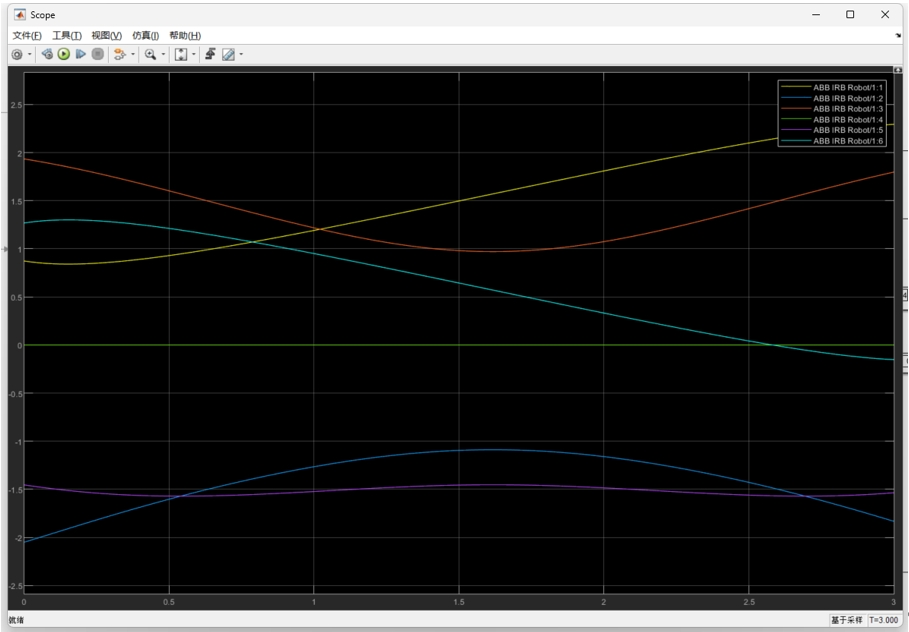
\includegraphics[width=0.5\textwidth]{Image/fig32.png}
    \caption{自定义运动下关节角度和电机侧加速度}
    \label{fig:26}
\end{figure}
\newpage
\subsection{基于模型的动力学仿真及PID控制}
在Simulink中进行机器人动力学仿真是一个复杂而庞大的过程,我们将图39所示的旋转关节参数设置中改为“Torque-Provided by Input”,如图\ref{fig:27}所示。这样相当于在旋转关节输入的是一个力矩(此处我们不考虑电机)。在前面动力学的分析中,我们通过“牛顿-欧拉”方法以及五次多项式可以规划出两点之间机器人的运动轨迹。与运动学仿真类似,在Simulink中可以输入以上计算结果的力矩进行运动仿真,当然,也可以输入一些常数(可以认为是常力矩值)来对系统进行一些测试。

\begin{figure}[htbp]
    \centering
    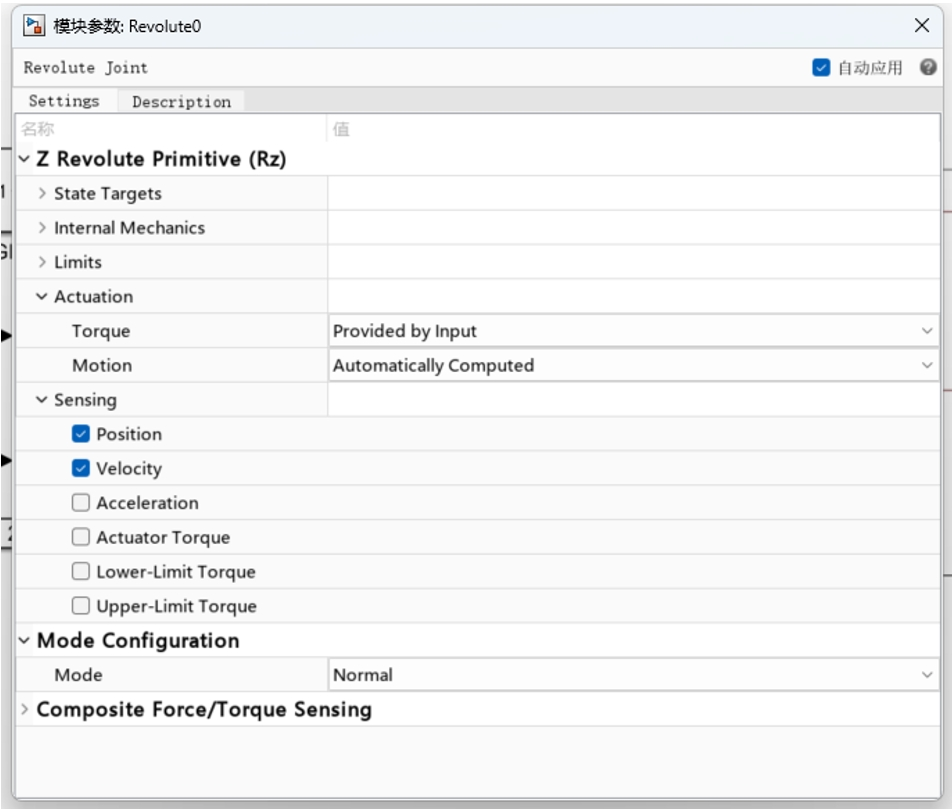
\includegraphics[width=0.4\textwidth]{Image/fig33.png}
    \caption{力矩输入模式}
    \label{fig:27}
\end{figure}

由于实际过程的动力学参数、机械结构参数、电机运动参数以及工况等因素过于多和复杂,我们的仿真不可能做到完美符合预期。因此我们从控制角度入手——通过末端绝对值编码器的反馈的位置信号,以期快速准确地达到预定的位置。对于许多机器人应用来说,控制系统的主要目标是确保关节达到预定的角度,而不需要严格的动力学模型。即使不考虑动力学,简单的PID控制器可以通过调节关节角度的误差来实现预期的定位。虽然PID控制器没有明确考虑动力学方程,但在某些情况下,适当调节PID增益可以隐式地补偿机器人系统的动力学特性。特别是在低速和低负载条件下,动力学效应对控制精度的影响较小,PID控制器能够提供足够的性能。引入PID后,系统局部如下图\ref{fig:28}所示。

\begin{figure}[htbp]
    \centering
    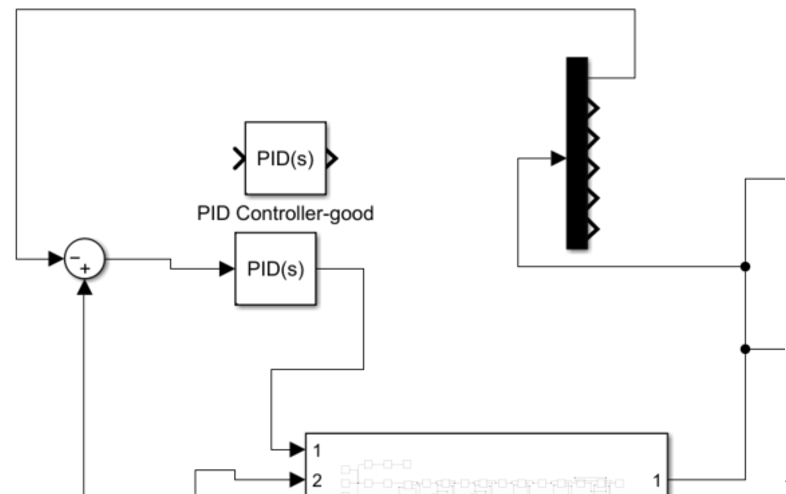
\includegraphics[width=0.6\textwidth]{Image/fig34.png}
    \caption{PID控制器的局部}
    \label{fig:28}
\end{figure}

由于实际过程的动力学参数、机械结构参数、电机运动参数以及工况等因素过于多和复杂,我们的仿真不可能做到完美符合预期。因此我们从控制角度入手——通过末端绝对值编码器的反馈的位置信号,以期快速准确地达到预定的位置。对于许多机器人应用来说,控制系统的主要目标是确保关节达到预定的角度,而不需要严格的动力学模型。即使不考虑动力学,简单的PID控制器可以通过调节关节角度的误差来实现预期的定位。虽然PID控制器没有明确考虑动力学方程,但在某些情况下,适当调节PID增益可以隐式地补偿机器人系统的动力学特性。特别是在低速和低负载条件下,动力学效应对控制精度的影响较小,PID控制器能够提供足够的性能。引入PID后,系统局部如图\ref{fig:28}所示。

\begin{figure}[htbp]
    \centering
    \subfigure[Without PID]{
    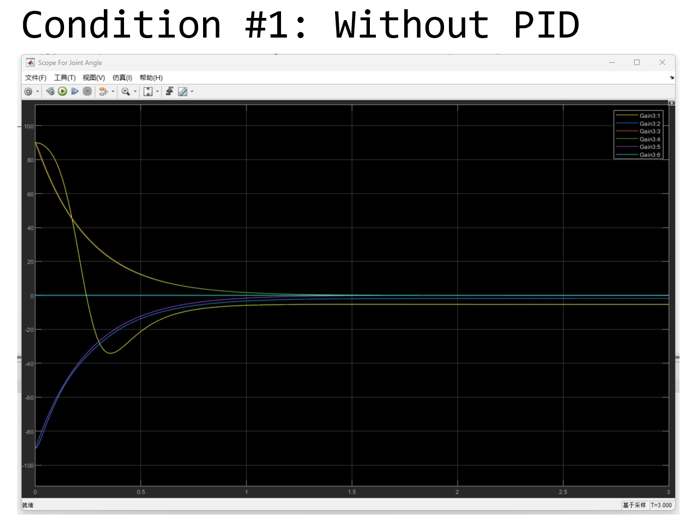
\includegraphics[width=7cm]{Image/fig35.png}
    \label{fig:29}
    }
    \quad
    \subfigure[$K_p=200,K_i=10,K_d=0$]{
    \includegraphics[width=8cm]{Image/fig36.png}
    \label{fig:30}
    }
    \quad
    \subfigure[$K_p=13.5,K_i=2,K_d=13.5$]{
    \includegraphics[width=7cm]{Image/fig37.png}
    \label{fig:31}
    }
    \caption{不同PID参数下的系统响应效果}
    \label{fig:28}
\end{figure}

没有PID控制的情况如图\ref{fig:29}所示。可以看到一号关节(黄色曲线)是一个典型的欠阻尼曲线,而且存在稳态误差。我们将此作为基本运动,对其进行调制。在图\ref{fig:30}中,我们使用了一个“不太优秀”的PID控制器,这个控制器的参数为$K_p=200,K_i=10,K_d=0$,它显著地增大了超调量,而且多了很多振荡不平衡的因素,不过最后稳态误差消除做的还比较理想。

在图48中我们调试出了一个较为优秀的PID控制器,该控制器在响应速度、稳态误差方面都做的很好,其$K_p=13.5,K_i=2,K_d=13.5$。具体的运动细节通过仿真很容易辨识出来,可以看到较差的控制器下振荡是很明显的,而表现优秀的PID使得关节响应准确、迅速。

\subsection{工业界机器人控制理论及部分复现}

这一部分我们主要从工业界主流的机器人控制理论出发,探讨工业界常见串联机械臂的动力学和控制问题。机器人的关节控制通常是“三环”,如图\ref{fig:32}所示。这三层控制环路层层递进,通过内层环路提供更快速和精确的控制响应,确保机器人关节运动的稳定性和准确性。

\begin{figure}[htbp]
    \centering
    \includegraphics[width=0.8\textwidth]{Image/fig38.png}
    \caption{机器人关节控制的“三环”结构}
    \label{fig:32}
\end{figure}

\textbf{电流环控制}:电流环控制是机器人关节控制的最内层环路,主要用于控制电机的电流。通过调节电流,可以直接影响电机的转矩,从而实现精确的力矩控制。电流环通常使用电流传感器反馈实际电流值,并与期望值进行比较,调整电压输出以减少误差,确保电机产生所需的力矩。这不是《机器人学》以及控制课的重点研究内容。

\textbf{速度环控制:}速度环控制是基于电流环之上的一个控制层,用于控制电机的转速。速度环使用速度传感器(如编码器)反馈电机的实际转速,与设定的目标速度进行比较,生成一个速度误差信号。这个误差信号再经过调节器(如PI调节器)处理,输出一个电流设定值,驱动电流环以调整电机的转速,实现对速度的精准控制。

\textbf{位置环控制}:位置环控制是机器人关节控制的最外层环路,负责控制关节的位置。通过位置传感器(如编码器或光学尺)反馈实际关节位置,与目标位置进行比较,生成位置误差信号。位置误差信号经过调节器处理,输出一个速度设定值,传递给速度环。速度环再将该设定值转化为电流设定值,逐层传递下去,最终实现对关节位置的精确控制。

因而我们本次大作业主要考虑速度环和位置环的控制模型搭建和测试。对于一个机器人关节,动力学上有一个优雅而简洁的方程进行描述:

\begin{equation}
    Q=M\left( q \right) \ddot{q}+C\left( q,\dot{q} \right) \dot{q}+F\left( \dot{q} \right) +G\left( q \right) +J\left( q \right) ^Tf
\end{equation}

式(39)中,Q代表广义驱动力,M是关节空间惯量矩阵,C是科里奥利力和向心力耦合矩阵,G是重力负荷,f是摩擦力,J是雅可比矩阵。在Peter Corke的机器人学工具包中,通过SerialLink.rne()方法(牛顿欧拉递归)可以从基座开始推算每个关节应该有的扭矩,具有O(N)的计算复杂性。

考虑一个电流控制的电机:
\begin{equation}
    \left\{ \begin{array}{c}	i=K_au\\	J_m\dot{\mathrm{\omega}}+B\omega +\mathrm{\tau}_c\left( \mathrm{\omega} \right) =K_mK_au\\\end{array} \right.
\end{equation}

其中$K_a$是运算放大器的跨导,$K_m$是电机的扭矩常数,电机的动力学模型可简化。其中$J_m$是电机的总惯量, $B$是电机的粘性摩擦系数,$\tau_c$是电机的库伦摩擦力矩。如果忽略库伦摩擦阻力项,对上式进行Laplace变换,可以得到:

\begin{equation}
    \left\{
        \begin{aligned}
            &sJ\Omega(s) + B\Omega(s)=K_mK_aU(s) \\
            &\frac{\Omega\left( s \right)}{U\left( s \right)}=\frac{K_mK_a}{J_ms+B}
        \end{aligned}
    \right.
\end{equation}

因此把电机简化为一个一阶系统模型。

\subsubsection{速度环控制}
通过上述分析,我们给电机的指令为:
\begin{equation}
    u^*=K_v(\dot{q}^*-\dot{q})
\end{equation}

因此搭建了一个速度环控制系统模型vloop.slx,如图\ref{fig:33}所示。

\begin{figure}[htbp]
    \centering
    \includegraphics[width=0.8\textwidth]{Image/vloop.png}
    \caption{速度环控制系统模型}
    \label{fig:33}
\end{figure}

将速度环封装在测试模型中(如图51所示),外部保留速度期望(desired speed)、干扰力矩($\tau_d$)的输入口,同时添加几个示波器用于检测关节速度和跟踪误差。需要一提的是,在图\ref{fig:33}中我们可以看到是有 $K_v,K_i$两个参数对反馈的信号进行调节,即我们提到的PI-Controller。测试模型如图\ref{fig:34}所示。

\begin{figure}[htbp]
    \centering
    \includegraphics[width=0.8\textwidth]{Image/vloop_test.png}
    \caption{速度环控制系统测试模型}
    \label{fig:34}
\end{figure}

接着在这个模型上进行测试,第一种情况我们假设没有干扰力矩,采用之前提到的连续梯形速度信号作为输入,可以得到下图\ref{fig:35}所示的结果。其中PI控制器的参数$K_p=1,K_i=10$。可以看到速度信号的跟踪水平一般,在速度的一阶导突变的地方跟踪性能会有一定的误差,考察Error图可以发现误差较大时,可以达到$1rad/s$。

\begin{figure}[htbp]
    \centering
    \includegraphics[width=\textwidth]{Image/fig40.png}
    \caption{零干扰力矩的速度环跟踪性能测试}
    \label{fig:35}
\end{figure}

但是对于实际的工程应用情景,机械手臂一定是存在重力作用的,因次每当我们在进行机械手臂的动力学仿真时一定要考虑重力力矩的影响。于是我们进行了第二组测试——添加干扰力矩,测试水平如图\ref{fig:36}所示。当添加的干扰力矩为$0.65N\cdot m$时跟踪误差将会更加显著($>3rad/s$),只是由于纵坐标的尺度不同,因此相对于图\ref{fig:35}其视觉上的误差更加小,实际上是更大的。

\begin{figure}[htbp]
    \centering
    \includegraphics[width=\textwidth]{Image/fig41.png}
    \caption{有干扰力矩的速度环跟踪性能测试}
    \label{fig:36}
\end{figure}

上述过程即为我们小组对速度环控制的研究。通常在工业界内有3中方法对机器人关节运动的跟踪性能进行改善:

\begin{itemize}
    \item \textbf{增加控制器增益}:通过增加控制器的比例增益$K_p$,可以提高系统的响应速度和稳定性,减小跟踪误差。但是增益过大会导致系统不稳定,产生振荡和过冲现象,使得系统不稳定。
    \item \textbf{增加积分增益}:在模型中引入积分增益$K_i$进行改善,做成如上图\ref{fig:33}中的PI控制器Velocity Controller。此时输入信号变为
    \begin{equation}
        \begin{aligned}
           \text{Time Domain:}\quad &u^*=K_v(\dot{q}^*-\dot{q})+K_i\int_{0}^{t}(\dot{q}^*-\dot{q})dt\\
           \text{Laplace Domain:}\quad  &U^*(s)=(K_v+\frac{K_i}{s})(\dot{q}^*(s)-\dot{q}(s))\\
           & (where \quad K_i>0)
        \end{aligned}
    \end{equation}

    这样的优势是将原来的0型系统变成了一个1型系统,因此对恒定的输入表现为0误差,但相应的缺点就是由于积分环节的作用可能会产生比较大的超调量。
    \item \textbf{加入前馈法}:对于一个实际的机器人模型,不管是PUMA560还是我们建的ABB-IRB-1200,其重力的干扰并不是未知的。我们可以计算估计或者使用一些上限/下限,预测干扰并消除它。值得一提的是,即使我们设置的前馈量不准确,前馈控制也能减少干扰的浮动。\textcolor{cherry}{也许这就是前馈控制系统的魅力所在吧。}
\end{itemize}

在工业界,前两种方法我们称为“\textbf{干扰抑制}”,后一种方法称为“\textbf{力矩前馈控制}”。让我们来观察一下力矩前馈控制的效果,系统框图如图\ref{fig:37}所示。

\begin{figure}[htbp]
    \centering
    \subfigure[力矩前馈控制框图]{
    \includegraphics[width=0.45\textwidth]{Image/力矩前馈.png}
    }
    \subfigure[力矩前馈测试系统]{
    \includegraphics[width=0.45\textwidth]{Image/力矩前馈测试.png}
    }
    \caption{力矩前馈控制系统}
    \label{fig:37}
\end{figure}

在测试环节加入了0.30的前馈量$\tau_{ff}$,对于同样的控制器参数,跟踪性能展示如图\ref{fig:38}所示,对比图\ref{fig:36},可以看到Error明显减少了(此时的纵坐标尺度相同),也成功地体现了前馈控制的作用.

\begin{figure}[htbp]
    \centering
    \includegraphics[width=\textwidth]{Image/fig42.png}
    \caption{力矩前馈控制速度环系统跟踪性能测试}
    \label{fig:38}
\end{figure}

\subsubsection{位置环控制}
可以这样理解:外环通过绝对值编码器检测关节位置,位置的误差为内环提供了速度要求。因此一个Ploop控制器应该嵌套了前一节中的速度环vloop,如图\ref{fig:39}所示。左上角为Ploop的外部测试,子系统ploop的结构如右下部分所示,其中包含了一个之前提到的vloop子系统。LSPB是一个集成好的轨迹发生器,规划关节1s内从0运动到1rad,并反馈回 $q,\dot{q},\ddot{q}$信息。

\begin{figure}[htbp]
    \centering
    \includegraphics[width=\textwidth]{Image/ploop.png}
    \caption{总集成的位置-速度环控制系统}
    \label{fig:39}
\end{figure}

测试这个装置,如图\ref{fig:40}所示。左侧的图是只使用比例控制的情况,类似于速度环内的控制,我们添加一项期望速度的前馈,可以得到良好的跟踪效果。

\begin{figure}[htbp]
    \centering
    \includegraphics[width=\textwidth]{Image/fig43.png}
    \caption{位置环控制系统测试}
    \label{fig:40}
\end{figure}

至此,控制部分的工作我们组就做了这些。虽然有限的课程内容里我们对这个机器人的控制所学不多,但它属实是一门充满了挑战、充满了未知的任务。我想这些工作也是对我们所学的一个完美谢幕,愿这份热情在心中永不熄灭,生生不息。

\newpage
\section{Reference}
[1]Peter Corke 机器人学、机器视觉与控制 MATLAB算法基础; Robotics, Vision and Control Fundamental Algorithms in MATLAB. 电子工业出版社, 2016. Print. 经典译丛·人工智能与智能系统,\href{https://doi.org/10.1007/978-3-319-54413-7}{https://doi.org/10.1007/978-3-319-54413-7}

[2]石青 (2019) MATLAB基础与机器人学应用; MATLAB foundation and its applications in robotics. 北京理工大学出版社

[3]克雷格 机器人学导论 = Introduction to Robotics: Mechanics and Control. 机械工业出版社, 2018. Print. 机器人学译丛

[4]李星辰,杨国庆,王宪,等.6轴工业机器人工作空间快速求解[J]. 机械科学与技术, 2023, 42(08): 1213-1220.DOI:10.13433/j.cnki.1003-8728.20220067.


\newpage
\section{Appendix}
烦请老师查看附件中的相关建模、代码、视频以及PPT,在这里汇总一下:
\begin{enumerate}
    \item \textbf{机器人建模部分}:内含有零件图、装配体图。以及我们在展示过程中的渲染图,含有匹配SoildWorks2018版本和2022版本的建模文件。渲染是基于2018版本的。
    \item \textbf{机器人运动学代码}:内含基础正逆运动学计算:基于工具包和不基于工具包;以及我们自己设计的圆弧运动\verb|DrawCircle.m|和\verb|CatchBall.m|;实现运动学解析逆解的代码文件为\verb|inkine8.m|。
    \item \textbf{机器人工作空间代码}:内含代码文件\verb|workspace_MonteCarlos.m|,使用的传统的Mento-Carlo方法;以及我们报告中所使用的\verb|MentoCarlo_Improved.m|,采用改进Mento-Carlo方法。
    \item \textbf{机器人动力学代码}:内含Jacobian矩阵的计算\verb|Jacobian.m|和正逆动力学求解代码。
    \item \textbf{机器人控制模型}:\verb|Model.slx|是我们的总模型,其中包含了我们建立的模型的slx格式,可进行仿真工作。\verb|Circle.m|是自定义信号的输入。\verb|vloop.slx|是速度环控制模型;\verb|ploop.slx|是位置环控制模型,是我们对工业机械臂关节控制的理论复现。
    \item \textbf{2024年6月4日课堂展示的PPT}。
    \item \textbf{Simulink-Configuration.pdf}.
\end{enumerate}
\end{document}
